\documentclass[a4paper,11pt]{article}

\usepackage[a4paper,width=15cm, left=3cm]{geometry}   %scale=0.7
\usepackage{supertabular}
\usepackage{url}
\usepackage{graphicx}
\usepackage{color}
\usepackage{float}
\usepackage{setspace}
\usepackage{longtable}
\usepackage{array}
\usepackage{listings}
\usepackage{latexsym}
\usepackage[pdftex]{hyperref}
\usepackage{enumerate}
\usepackage{enumitem}
\usepackage{needspace}

\spacing{1.213}

\setlist[itemize]{noitemsep} 
%\setlist[itemize]{itemsep=1cm}

\usepackage[tight,footnotesize]{subfigure}

\usepackage{changepage}   % for the adjustwidth environment

\usepackage{showframe} % show page borders
\renewcommand*\ShowFrameLinethickness{.2pt}
\definecolor{palegray}{gray}{0.8}
\renewcommand*\ShowFrameColor{\color{palegray}}

\usepackage{listings}

\lstdefinelanguage{Java} {
    basicstyle={\fontsize{10.4}{12}\ttfamily},columns=flexible,mathescape=true
}

\lstdefinelanguage{json} {
  basicstyle={\fontsize{10.4}{12}\ttfamily},
  breaklines=true,language=java,columns=flexible, breakatwhitespace=true,
}

\lstdefinelanguage{config} {
  basicstyle={\fontsize{10.6}{12}\ttfamily},
  breaklines=true,columns=flexible, breakatwhitespace=true,
  frame=single, basicstyle=\scriptsize\ttfamily
}



\newcommand{\code}[1]{%
  \vspace{0.8em} \small{ \texttt{#1}} \normalsize \vspace{1em}%
}

\newcommand{\smalltt}[1]{%
  \footnotesize{ \texttt{#1}}%
}

\renewcommand{\appendix}[1]{%
   \newpage \section{#1}%
}


\definecolor{palegray}{gray}{0.8}
\definecolor{midgray}{gray}{0.6}

\newcommand{\hr}{%
  \needspace{5\baselineskip} \noindent{\color{midgray}\noindent\rule{\textwidth}{1pt}}%
  \vspace{\glueexpr\baselineskip - 4pt plus 0pt minus 15pt\relax}
}

\usepackage{tikz}
\usetikzlibrary{shapes,positioning,matrix}

\begin{document}

\title{A Guide to User Space Routing -- \\
VLSP -- The Very Lightweight Network \& Service Platform}
\date{Jan 2018}
\author{Stuart Clayman}
%svjour2
%\subtitle{Very Lightweight Network \& Service Platform}
%\institute {Dept. of Electronic Engineering, University College London}


\maketitle


\begin{abstract}
This document gives an overview of the \emph{VLSP}
framework.
We have designed a  testbed called
the \emph{Very Lightweight Network \& Service Platform} based on this framework.
It uses a set of Virtual Routers and Virtual Network Connections to
create a test  environment which can easily accommodate
 (i) fast setup and teardown of a Virtual Router,
and (ii) fast setup and teardown of a Virtual Connection.
Each Virtual Router can run small programs and service elements. 

\smallskip
The document describes the platform itself and the components in more
detail.
The usage and startup of the platform is presented together with the
configuration options.

\end{abstract}



\section{Introduction}
\label{chap:intro}
This document gives an overview of the \emph{VLSP}
framework - sometimes called  \emph{User Space Routing} as it does
everything in user-space.
We have designed a  testbed called
the \emph{Very Lightweight Network \& Service Platform} based on this framework.
It uses a set of Virtual Routers and Virtual Network Connections to
create a test  environment which can easily accommodate
 (i) fast setup and teardown of a Virtual Router,
and (ii) fast setup and teardown of a Virtual Connection.
Each Virtual Router can run small programs and service elements. 

The platform consists of a number of virtual routers running
as Java virtual machines (JVMs) across a  number of physical machines.
The routers are logically independent software entities which, as with
real routers, communicate with each other via network
interfaces.  The network traffic is made up of datagrams, which are
send to and from each router. The datagrams are not real UDP
datagrams, but are our own virtual datagrams (called USR datagrams) which are
used.

The platform has three components, the major one of 
which is the ``Router'' itself.  They are complemented by a
lightweight ``Local Controller'' which is similar to a hypervisor and has the role of sending instructions to start up 
or shutdown routers on the local machine and for routers to setup or
tear-down connections with other virtual routers.  The whole testbed
is supervised by a ``Global Controller''.  
This software entity is like a combined Virtual Infrastructure Management (VIM) / Orchestrator,
%does not exist on a real running virtual router system but,
and has the role of a
co-ordinator.  That is to say, it informs 
Local Controllers when to start up and shut down routers and when to 
connect them to each other or disconnect them from each other.
%In a real system these decisions might be made by the management
%system.


Since its inception, VLSP has been used in many experimental
situations that have benefited from its flexibility, adaptability,
lightweightness, and scalability.
VLSP achieves better simplicity and non-functional characteristics
over using a hypervisor running a standard virtual machine and
standard OS (i.e. improved scalability; lower resource utilization;
quicker startup speed; reduced heaviness; eliminate the issue where
most of the router functionality is not needed; and more networking
flexibility).  VLSP is fully distributed and modular. This has
been achieved, as the management components as well as the host
controllers and the virtual entities themselves can be deployed across
any number of physical hosts interacting via REST calls.


\noindent From the experimental usage of VLSP we have determined:
\begin{description}[leftmargin=1em,labelindent=0,itemsep=3pt]
\item \textit{What is VLSP good for?}

\begin{itemize}
\item Testing and evaluating alternative SDN / NFV scenarios
\item Mid scale tests of network software written in Java (100s and likely 
1000s of virtual routers).
\item Testing software robustness to ``unexpected" network conditions
(sudden ``rude" start up/shut down exposes software deficiencies).
\item Testing software robustness to unreliable networks.
\item A compromise between simulation (realism questionable) and large
testbed (requires many physical machines).
\item Comparing simulation with testbed results
\end{itemize}

\item \textit{What is VLSP \emph{not} yet good for?}

\begin{itemize}
\item It is not optimized for forwarding performance, compared to a real router it routes packets at a slower speed and uses more overhead (i.e. due to the focus on the support of new network management and control features).
\item It is difficult to support facilities and protocols that rely on maximum bandwidth
  calculations, e.g. traffic engineering algorithms estimating
  the link bandwidth.
  \item The direct interaction with or the driving of hardware interfaces
  is out not currently addressed. % in the current implementation.
%  has space for performance improvements.
\end{itemize}

\end{description}



\subsection{Motivation}

There were many motivations for designing and building the \emph{User Space Routing}
framework.  These were accumulated from experience on various research
projects, including RESERVOIR which investigated running services in virtual machines, and
the AutoI project, which investigated the virtualization of network
elements.
It was found that the use of a hypervisor and the associated virtual
machines did work as expected and as required, however, there were
some issues that hindered various experimental situations.

We found that using a hypervisor and virtual machines added only 5\%
to 10\% overhead to operations, compared to running the same
operations in the physical machine, which is most cases was entirely
acceptable.  The small loss of efficiency was easily overcome by the
flexibility of having virtual machines.
In terms of experimental and research issues, some were general issues
and others were specific to the domain. We found the following general
issues:

\begin{itemize}[itemsep=1ex]
\item the number of virtual machines that can run on a physical host
  is limited.  This can be due to the actual resources of the physical
  machine that need to be shared (such as the number of cores and the
  amount of memory available), together with the switching
  capabilities of the hypervisor.

\item the speed of startup of a virtual machine can be quite
  slow. Although virtual machines boot up in the same order of
  magnitude as a physical host, there are extra layers and
  inefficiencies that slow them down.  Also, if many virtual
  machines are started concurrently, then we observe that the physical
  machine and the hypervisor thrash trying to resolve resource
  utilization. 

\item the size of a virtual machine image is quite large.  A virtual
  machine has to have a disc image which contains a full operating
  system and the applications needed for the relevant tasks.  To start
  a virtual machine, the operating system needs to be booted and then
  the applications started.  So every virtualized application needs
  the overhead of a full OS.

\end{itemize}

\noindent and we found the following issues that were more domain
specific:

\begin{itemize}[itemsep=1ex]

\item in terms of virtual networks, and virtualized routers in
  particular, we observered that 95\% of the router functionality we
  never utilized in any of the experiments that were run.  Although
  software routers such a XORP and Quagga allow anyone to play and
  evaluated soft networks, the overhead of a virtual machine, with a
  full OS, and an application where only 2\% is used, seems to be an
  ineffective approach for many situations.

\item when trying to configure the IP networking of virtual machines
  and virtual routers, there are some serious hurdles.  The virtual
  machines do not talk directly to the network, but go via the
  hypervisor.  The hypervisor has various schemes for connecting
  virtual machines to the underlying network, each of which has
  different behaviour.  In most situations where experimentation of
  virtual routers is required, there needs to be a large range of IP
  addresses available.  However, this is often hard to come by.
  We found that the limits of addressing, the IP networking
  configuration, and virtual machine to virtual machine
  interoperability a hindrance to network topology and network flexibility.


\end{itemize}

\noindent It was felt that to make more progress in the area of
dynamic and virtual networking experimentation and research, we needed
to design and build a testbed that did not have these limits, but still retain 
virtual machine technology.

The main goals of the testbed over using a hypervisor running a
standard virtual machine and standard OS are to have:

\begin{itemize}
\item better scalability
\item lower resource utilization
\item quicker startup speed 
\item reduced heaviness 
\item eliminate the issue where 95\% of the router functionality not needed
\item more networking flexibility
\end{itemize}

\noindent The choice was made to write our own simple router with
simple service capabilities, in Java, that
could run in a Java Virtual Machine (the JVM).

\subsection{Benefits}

The benefits of a lightweight VM that includes a simple router and the
basic capabilities of a service component are: 

\begin{itemize}
\item it is possible to run many more routers on a host
\item it is easier to test scalability and stability
\item it is possible do enhanced monitoring and management evaluations
\item it provides a different way to do virtual networks: we can
  create arbitrary topologies using virtual routers 
\item it is possible to do more evaluations of network management and
orchestration functions by not
using complete routers and full services
\end{itemize}

\noindent In general, it is a more effective platform for
experimenting with many aspects of virtual networks, management of
virtual elements, and orchestration experiments.

The VLSP integrates and unifies management of networks,
compute, and services into a
single platform.
The whole system, including a lightweight virtual router, was
designed and built from scratch to enable flexible experimentation of
virtual infrastructures.  VLSP has the following
advantages:

\begin{description}[leftmargin=1.5em,labelindent=0,itemsep=3pt]

\item \textit{Lightweight virtual router implementation:}
to allow evaluation of diverse scenarios, including the
testing of various management lifecycle schemes.
It allows the testing of software 
robustness to ``unexpected" network/node conditions
(such as sudden start up/shut down events exposing software deficiencies),
where a virtual element can disappear at run-time under management control.
VLSP is a
positioned between simulation (realism questionable) and large testbed
(requires many servers).
Lightweight routers being deployed and managed in a distributed environment, suitable for reliability and scalability tests.

\item \textit{Distributed infrastructure implementing logically-centralized management and control:}
By employing the SDN paradigm, while
avoiding overflowing centralized components,
to support optimizations,
based on centralized decisions using a global system picture 
 derived from an integrated monitoring infrastructure based on
Lattice \cite{lattice}.
It also supports flexible and adaptable service provisioning, plus aspects
beyond traffic engineering, 
(e.g. adaptable service deployment /
operation, optimized distributed node placement etc).

%Hierarchical and distributed control components that perform scalable and logically-centralized network control, without overloading centralized software nodes.

\item \textit{Experimentation on management:} 
 to focus on the experimentation of distributed management and
control components of software-defined infrastructures rather
than data plane performance.
Along these lines,
 VLSP brings the following benefits:
 (i) more routers can be deployed
 on each host, making it easier to test scalability and stability;
 (ii) enhanced distributed management, control and monitoring evaluations can be carried out, which is difficult to achieve in a running environment using a number of deployed data centers;
(iii) arbitrary topologies can be created using virtual routers, providing a more general way to form virtual networks; 
(iii) suitable for both experimentation with virtual networks and
lightweight virtual servers; and (iv)  supports experiments with
dynamic topologies (such as migratable virtual routers)
 and mobile extensions of the network infrastructure). 

\item \textit{Support of integrated SDN and NFV environments:}
to uncover the potential of
virtualized SDN solutions and NFV deployments, in a naturally
integrated way, with common management and control
facilities.

\item \textit{JVM based Runtime Environment:} The evaluation of
 network topologies allowing hundreds or thousands of virtual
 nodes (routing or compute), using
 software written in Java. Each node resides in its own virtual
 machine, and so is independent of and secure from all other virtual nodes.
 The software execution environment, available on all nodes, allows the deployment of diverse network control components. Existing Java code can be quickly ported to run on our
 software router (our experience is from two or three hours, to a few days for relatively
 complicated software packages). Deployment of virtualized devices over heterogeneous hardware and software environments due to the very wide support of the JVM technology. 


\end{description}


\section{The Platform}
\label{chap:platform}

In this section there is a more detailed overview of the platform
itself.
VLSP provides a complete environment from the
\emph{protocol stack} up to the \emph{service management} level,
including a tailor-made monitoring facility. Consequently, we are able to
experiment with new complete 5G network management and control
facilities over virtual networks based on our lightweight virtual
entity resembling both servers and routers.

 VLSP is a distributed management
infrastructure that has centralized functionality and is
responsible for the setup, configuration, optimization, and shutdown
of network entities.
 It has been implemented for the
purpose of testing and evaluating various aspects of managing  highly dynamic virtual
environments, in particular  the 6 aspects of:

\begin{adjustwidth}{\parindent}{}
\begin{enumerate}[label=(\roman*),noitemsep]
\item efficient service function,
\item optimized service function availability,
\item service and VNF lifecycle automation,
\item service placement automation,
\item efficient resource utilization, and
\item  dynamic resource up/down scaling (elasticity).
\end{enumerate}
\end{adjustwidth}

\noindent VLSP is a testbed that consists of a large number of virtualized entities which
execute on a number of physical machines.
The entities are logically independent software entities that
communicate with each other via network interfaces. 
The testbed has been validated
for some of these aspects in previous work we have undertaken on
virtualized and highly dynamic networks.

The VLSP set up has various components described in this section
and include:

\begin{adjustwidth}{\parindent}{}
\begin{enumerate}[label=(\roman*),noitemsep]
\item a supervisor and experimental
controller realizing the basic functionalities of an Orchestration
Layer  / Virtual Infrastructure Management (VIM) called the  \textit{Global Controller};

\item per-host \emph{Host Controllers};  and

\item the \emph{virtualized entities}, which run inside a JVM.
\end{enumerate}
\end{adjustwidth}

\noindent VLSP is configured by the \emph{Global Controller} running 
on one physical server, and the \emph{Host Controllers} running on
physical machines that host virtual entities.
Under control of the
\emph{Global Controller}, the individual \emph{Host Controllers}
start or interact with virtual entities when needed. The choice of
\emph{Host Controller} is decided by the \emph{Placement Engine},
which uses an algorithm to determine the \emph{best} physical machine
to deploy the new virtual entity.  The \emph{Global Controller} also
sends requests, via a \emph{Host Controller}, to 
connect virtual routers together via virtual  links.

In order to manage the challenging and dynamic infrastructures of
virtual networks there needs to be a monitoring system which collects
data and reports on the behavior of both the physical resources
(e.g. CPU usage, memory usage) and the virtual resources
(e.g. utilization level of the virtual links). The monitoring data
items are sent to the \textit{Global Controller} components. The
monitoring information is used to take decisions regarding network
strategies and enforces these decisions. The monitoring system
\emph{Lattice} is used as has been proven to be ideal for the task of
collecting monitoring data for various types of dynamic network
environments.  Each virtual entity has at least one probe that can
generate data. Monitoring data is also collected from each \emph{Host
  Controller}. All of this monitoring data is send to the \emph{Global
  Controller}, and it is the data that is used by the \emph{Placement
  Engine} for determining where a new virtual entity is placed.


\subsection{Main Function Elements}



The main elements of the Platform are the Orchestration
Layer  / Virtual Infrastructure Management (VIM) called the  \emph{GlobalController},
the per-host \emph{Host Controllers}, called the \emph{LocalControllers}, and the \emph{Routers}.  These are each
explained in further detail below.

The main elements can be found in the following table.

\begin{longtable}{ | p{5cm} | p{9cm} | }

\hline
\textbf{Name} & \textbf{Description} \\
\hline
Host Controllers & The host controllers execute on every physical
machine and manipulate and configure virtual routers, links and virtual
router applications. \\
\hline
Monitoring System & The monitoring system, comprising probes that are tiny configurable applications
probing the software or hardware for monitoring data, as well as the
data consumers. \\
\hline
Event Management & It is responsible for the runtime operation,
including support for event-based notifications and time scheduling. \\
\hline
Virtual Router Protocol Stack & The lightweight network protocol stack
of the VRs.  \\
\hline
Virtual Router Application Environment & The application environment that hosts VR applications. \\
\hline
Virtual Link Functionality & The functionality of the virtual links,
including link weighting and other configuration options. \\
\hline
Virtual Machine for Virtual Router and Application Functionality & A
virtual machine with the virtual router and the relevant applications
functionality. \\
\hline

\end{longtable}

\noindent There is one \emph{VIM} for the platform, and it has the
following functions:

\begin{itemize}
\item it starts and stops the LocalControllers
\item it acts as a control point for the platform by sending out commands, 
\item it acts as a management element for the platform by collecting
  monitoring data and enabling reactive behaviour 
\end{itemize}

\noindent The Virtual Infrastructure Management (VIM)  can run on the same host as a
LocalController, or in a large setup it can run on a separate host.
The VIM component is responsible
for the management and lifecycle of the virtualized elements that will
be used within a network, particularly virtual network elements. As
the virtual elements are not physical themselves, but exist on top of
physical elements, their lifecycle and their management needs to be
approached carefully to ensure continued operation and consistency.

The virtual network elements, which exist on top of physical networks,
can be setup with arbitrary topologies and with an arbitrary number of
end-points. The virtual links in a virtual topology are eventually
mapped onto physical links in the underlying network. A virtual link
may span multiple physical links, and cross many physical routers, or
it may span a single physical network link. New virtual links can be
added or can be removed from a virtual network dynamically at
run-time.

The virtual networks are very flexible and adaptable, and generally
have few limitations, except that a virtual link cannot support more
traffic and higher-data rates than the underlying physical
links. Furthermore, a whole virtual network can be shutdown as needed,
if the applications that use it no longer need the network. Such a
shutdown frees resources from the underlying physical network.

%% The full management of virtual networks on physical networks requires
%% the matching and analysis of the flow rates on the virtual links to
%% the flow rates of the underlying physical links. It is important to
%% ensure that the physical links are not congested with too many virtual
%% links. Also, the allocation and mapping of virtual links must take
%% into account the current state of the physical network and the current
%% virtual networks. However, if a situation arises where a
%% re-configuration is required, the virtual network management should be
%% capable of mapping a virtual link across different physical links at
%% run-time, but leave the virtual topology intact.

The VIM component has a seemingly simple task, but in reality the
management requires continual monitoring, analysis, and adaption of
the virtual elements to the physical elements. As all of these virtual
elements are distributed, the management is a complex task.
The VIM interacts with the virtual network
elements that will be present in a running virtual network. All of the
elements of the VIM component constitute a fully distributed system,
whereby an element or node can reside on any host. A full virtual
network can be instantiated on a single machine, for demonstration or
testing purposes, or instantiated across multiple servers, in a full
deployment situation.

The VIM directly controls the lifecycle of each virtual element, by
collecting knowledge on the status of physical resources in order to
determine where a virtual element can be created. The virtual network
element will be created, managed, and shutdown by lifecycle phase of
this component.

Due to the dynamic nature of virtual elements and because they can be
disassociated from the physical elements they are mapped to, it is
possible to do a live adaption of a virtual element from one physical
host to another physical one, at run-time.

The VIM controller acts as a control point for managing the virtual
elements. This block accepts all its input via the VIM REST interface
from other management applications / network services. The monitoring
engine acts a collection point for the monitoring data needed to keep
the management functions running. Control commands are sent to
the VIM and they are either acted upon immediately or are passed to
the corresponding Host Controllers.

The main VIM elements can be found in the following table.
\begin{longtable}{ | p{5cm} | p{9cm} | }

\hline
\textbf{Name} & \textbf{Description} \\
\hline
VIM Controller & It is the heart of the component, providing the
central control of the VIM operations. \\
\hline
Scripting Engine & VIM can be configured using Closure
scripting. \\
\hline
Monitoring Engine & It is the main monitoring component of the
infrastructure, i.e., collecting \& manipulating measurements from the
monitoring probes residing at the virtual entities. \\
\hline
Virtual Entities / Topology Configurators & These functions are responsible for the configuration of virtual routers, links and topologies, supporting different levels of abstraction. \\
\hline
Configuration Actuators	& The Virtual Entities / Topology
configurators communicate with the configuration actuators which in
turn enforce the configuration changes through the LNH's host
controllers. \\
\hline
\end{longtable}


There is one \emph{LocalController} for each physical host that needs
to execute virtual routers.  A LocalController has the following
functions:

\begin{itemize}
\item it starts and stops virtual routers
\item it tells routers to create and remove virtaul network
  connections
\item to get or set attributes on routers or links
\end{itemize}

\noindent A LocalController is similar to a hypervisor in a normal
virtualization environment, as it has a role of stopping and stopping
virtaul machines.

Within the platform, many \emph{Routers} can be created.  These
virtaul routers behave like a real hardware router, with the caveat
that they have much simpler functionality.

\begin{figure}
    \centering
    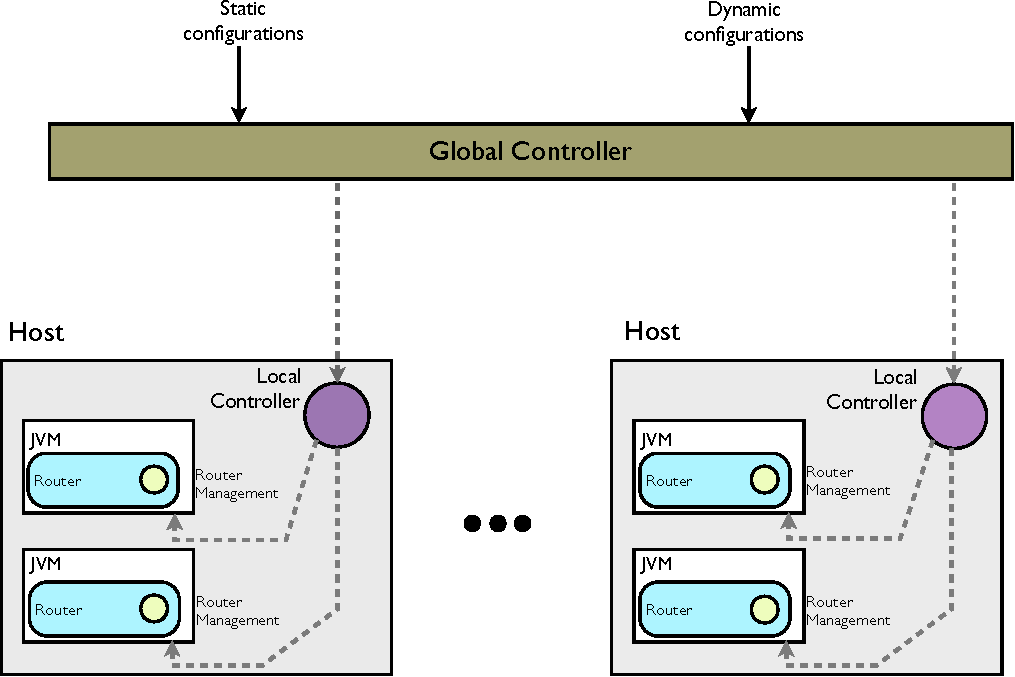
\includegraphics[width=13cm]{images/architecture}
    \caption{General Architecture}
    \label{usr-architecture}
\end{figure}

In figure \ref{usr-architecture}, the relationship between these
elements is shown. There is the VIM / GlobalController, shown in brown, which can take
various configurations in order to setup and control a run.  These
configurations can be static configurations, where there is a fixed
topology, or dynamic configurations, where the topology of the network
and the number of links changes on-the-fly under the control of the
GlobalController.

The GlobalController interacts with various LocalControllers.  This
interaction path is shown as a dotted line.  A LocalController,
shown in purple,
executes on each physical host that participates in the platform.
Each LocalController takes requests from the GlobalController and
takes the required action.  This can be to start or stop a virtual
router, to create or remove a virtual link, to get or set attributes
on routers or links.

To start a new Router, shown in blue, the LocalController on the
relevant host will start a new Java Virtual Machine, shown in white,
executing the specific Router code.  The router has various elements,
which will be discussed later, however for this discussion the most
important one is the Router Management element, shown in yellow.  Once
a Router is up and running, the LocalController interacts with it via
the Router Management interface.  It is using this interface that
commands and requests for the Router are sent by the
LocalController. This path is also shown via a dotted line.


Although there is a considerable amoount of infrastructure in the
platform dealing with control, the main aim of the platform is to
create a topology of virtual 
routers.  These routers execute on a set of hosts, with virtual links
between the virtual routers. 
In figure \ref{usr-hosts}, we see how the topology of virtual routers
and virtual links manifests itself across multiple hosts, three in this
case. 

\begin{figure}[h!]
    \centering
    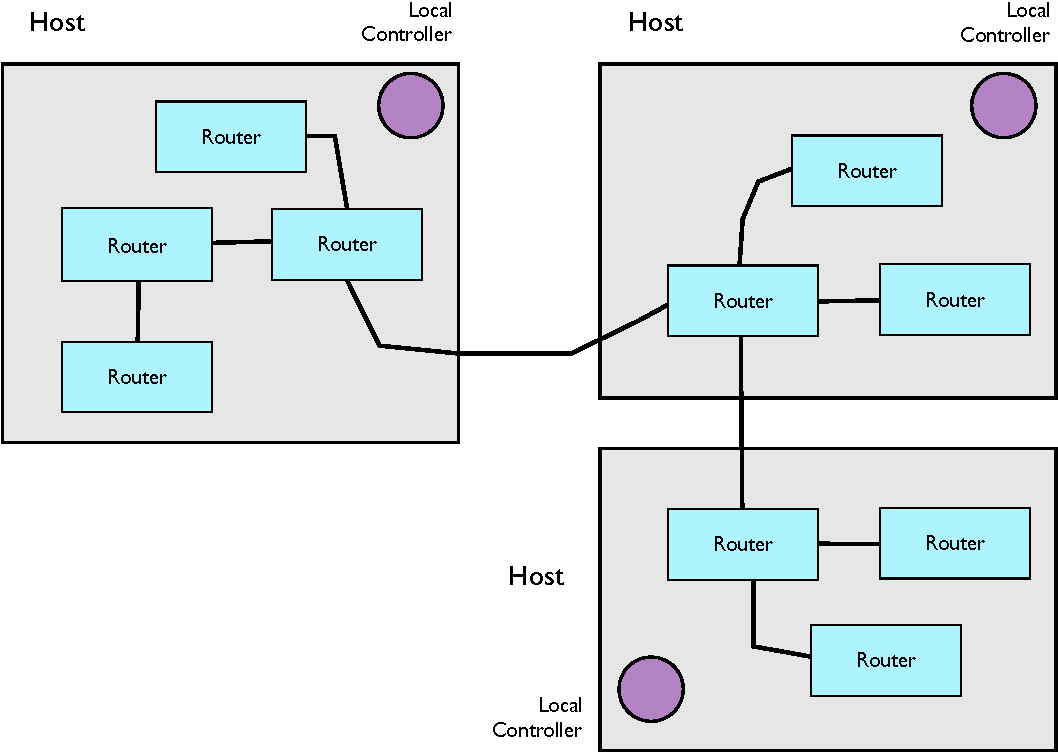
\includegraphics[width=13cm]{images/hosts}
    \caption{Hosts with Virtual Routers and Virtual Links}
    \label{usr-hosts}
\end{figure}

An alternative view of the platform where the hosts are not shown, but
there is the control path and the virtual routers and virtual links is
shown in figure \ref{usr-control}.
Control propogates from the GlobalController, via the
LocalControllers, to the Routers.
The topology of Routers is connected by separate virtual links.

\begin{figure}[h!]
    \centering
    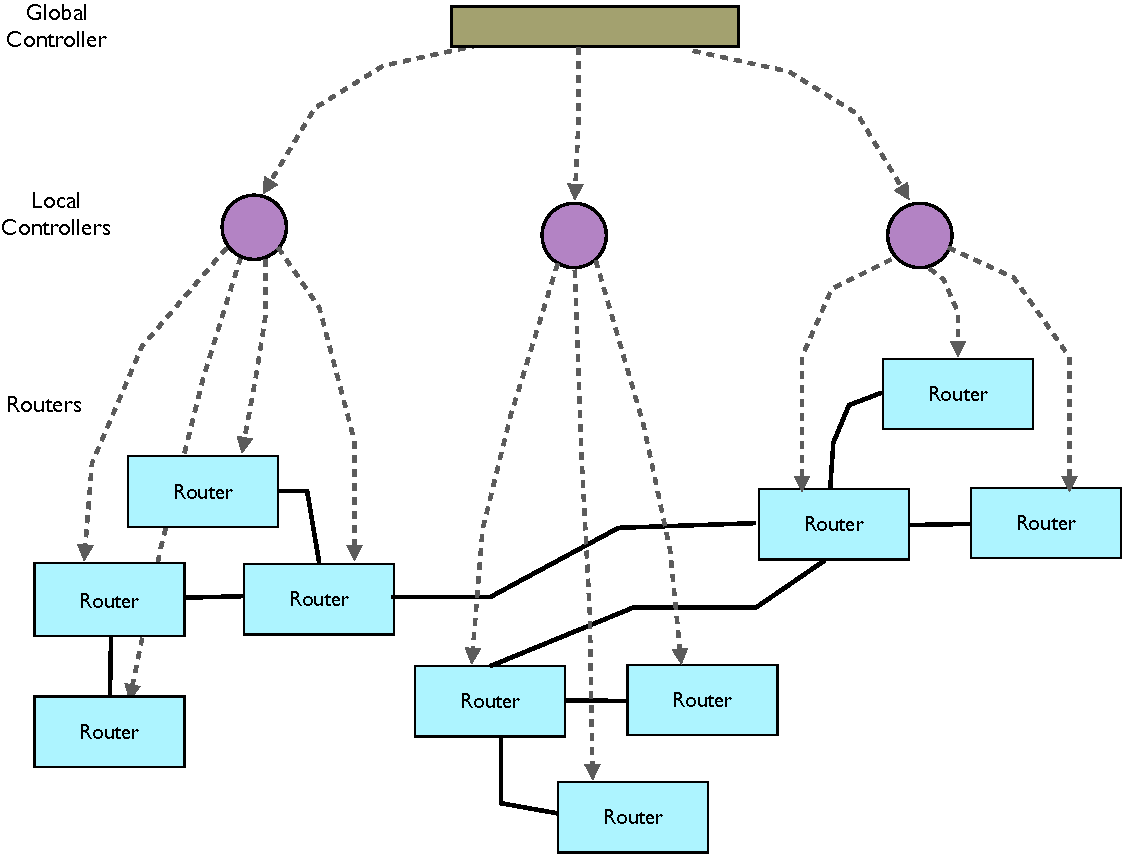
\includegraphics[width=13cm]{images/control-path}
    \caption{Full Connectivity with Control Path}
    \label{usr-control}
\end{figure}


\subsection{Main Platform Functions}

The main functions of the  Very Lightweight Network \& Service
Platform are outlined in this subsection. 
The platform uses a set of Virtual Routers and Virtual
Network Connections to create a test environment which can easily
accommodate:
\begin{itemize}
\item fast setup / teardown of a Virtual Router
\item fast setup / teardown of a Virtual Connection
\item each Virtual Router can run small programs / service elements
\end{itemize}

\noindent These are explained in more detail in the following sections.

\subsection{Routers}

The software virtual router is implemented in Java and is a relatively complex 
software entity.  The routers hold network selections to the other virtual
routers they are aware of and exchange routing tables to determine the 
shortest path to each other router.  Datagrams are sent between routers
and queued at input and output.  A system of virtual ports (like the 
current transport layer ports) are exposed with an interface very similar
to standard ``sockets".  Virtual services can be run on the virtual
routers and listen and send on the virtual sockets. 
The datagrams themselves, have headers 
with a source address, destination address, protocol, source port, destination port,
length, checksum and time to live -- many of the features of real UDP
packets are replicated.  

\subsection{Routing and packet transmission}

Routing in these virtual routers is distance-vector based.  To prevent routing storms
minimum times between table transmissions are set.  In addition, because
the experiment here demands a certain ``churn" of virtual routers
then addresses which disappear permanently must be dealt with.  In distance
vector routing it is well-known that dead addresses can leave routing loops.
This is dealt with in the current system by implementing time to live
(TTL) in packets and
also implementing a maximum routing distance beyond which a router is assumed
unreachable and removed from routing tables.

Virtual services can run on the routers.  Naturally the only important
virtual services for the purposes of our evaluations are networked
services.  The services
tested include simple network test protocols such as ping and traceroute and
ftp style send and receive services.
The major software used, however, is the Lattice monitoring framework developed for
 RESERVOIR.  
The virtual services can listen on virtual ports and send datagrams to any
address and virtual port.

Datagrams are queued both inbound and outbound, the outbound queue is blocking 
in order that transmitting services can slow their sending rate.
The inbound queue is tail-drop so that when too much traffic is sent drops
will occur somewhere.  TTL is decreased at each hop and, on expiry, a "TTL
expired" packet is returned -- this allows the virtual router system to
implement traceroute as a virtual service.  Virtual routers in the 
system send all traffic including routing tables and other control messages
via network sockets.  Control messages (routing tables, echo, echo reply,
TTL expired and so on) are routed in the same way as data packets on a
hop by hop basis using the routing tables.  
Datagram transmission is UDP-like in this
iteration of the system, that is, delivery is not guaranteed and a failure
to deliver will not be reported to the service (although if the router
on which a virtual service runs
has no route to the host this can be reported to the service).

\subsection{Start up and tear down}

Start up and tear down for routers is scheduled by the Global Controller
and directly performed by the Local Controller which resides on each
physical machine as the virtual router.   The
virtual routers would operate perfectly well without such a controller,
for example, if they were set up and connected manually or by some other
distributed control system.  The Local Controller is necessary to
spawn off new routers on a machine.
In addition, the Local Controller is used here to
pass on Global Controller commands to shut down or connect virtual
routers.  

\subsection{Virtual Services / Applications}

Each virtual router has a socket interface by which services and
applications can be written.  All networking interactions are done using
our USR Datagram layer, which is very similar to the standard Java
socket and datagram interface.
Each service can open a socket on a given address and port, and
can send traffic to an address and a port.

By having our own virtual datagram layer we could control all the
networking within the virtual router.  However, by making the socket
and datagram interface very similar to the standard Java one, we were
able to utilize existing Java software which has a standard UDP
mechanism.

As an example of easy re-used of existing software, consider that it
took just a few hours to port the Lattice monitoring
framework onto this new platform.  We wrote an implementation of the
data plane using USR instead of UDP.  In terms of the source code,
there are few differences between each implementation.

\subsection{Monitoring}

The monitoring software used in VLSP is called Lattice and has been
used for monitoring virtualised services in federated cloud
environments, for monitoring virtual networks, and as the
monitoring system for an information management platform that
aggregates, filters, and collects data in a scalable manner within
virtual networks. Lattice, which is also an open-source
software, has been proven to be ideal for the task of collecting
monitoring data for various types of dynamic network environments.

Each virtual router has a set of probes which generate data for
virtual link usage, cpu / memory usage per thread, and virtual
applications resource consumption. This data is sent to the Monitoring
Engine of the Global Controller which processes it. This data is
used by the Placement Engine for determining where a new virtual
router is placed. 

\subsection{REST API for Dynamic Programmable Control}

A dynamic programmable control environment allows the definition of
scenarios, resources, or other software entity parameters using
appropriate functions via a REST API. In our case, we use a Java
client or one written in the Clojure language
for the dynamic configurations. This allows us to perform fully
Software-Defined Operations using a functional language that has an
expressive representation of the configuration settings, while being
very brief.

\subsection{Event Engine for Probabilistic Experiment Control}

Many experiments that are undertaken in the networking domain are
based on arrival rates that are taken from a probability
distribution. Within VLSP we have an \emph{event engine} that can generate
events to create a router, destroy a router, create a link, and delete
a link, all based on probability distributions.

For any particular run
we can specify these distributions together with their associated
parameters in an XML configuration file. The options for the
distribution are set 
in a Type field as one of: Uniform, Exponential, LogNormal, or
PoissonPlus, matching well-known topology models. Fur- thermore, we
are providing pre-defined configuration files with realistic
topologies, e.g. for data centers. 

\subsection{VLSP Visualization}

One of the management tools we have built for VLSP is a Network
Visualization tool. It takes a logical graph view of the virtual
topology, including the routers and the links, and presents a
visualization graph by using the graphviz tool. From data held by the
Orchestration Controller, a version of the network is generated in the
dot language that graphviz uses. As dot is very flexibile, it is easy
to create extensions to the visualizations which include the virtual
applications that execute on the routers. Furthermore, we are able to
present key nodes in different shapes and colours in order to
highlight the different features of a topology. As an example,
consider the topology on the cover which represents a partial snapshot
from one of our experiments. Those with a similar colour are 
logically connected for managing the same data streams, and those
nodes represented as a diamond shape are running a Data Proxy
application. It allows us to see how data management applications are
deployed across the whole topology. 


\section{Usage}
\label{chap:usage}

In this section the usage of the platform is described.  We show how
to start up the platform and how to configure different runs.

Remember that there are 3 main components of the platform:

\begin{itemize}
\item the Global Controller
\item Local Controllers
\item Routers
\end{itemize}

\noindent Within a run, there will be one Global Controller, which controls the
run, a Local Controller on each physical machine that participates,
and a set of Routers that run on the physical machines.

To start the whole VLSP system, we execute the \emph{Global Controller} and pass in an \textsc{xml} file which has the configuration options
for each particular run, specifying
 a Java class
called:  \lstinline[language=Java]$usr.globalcontroller.GlobalController$.
The options include information such as the
ports to listen on; the hosts that the \emph{Host Controller} is to execute
on and its associated ports; its monitoring elements; the placement engine to use; and other
virtual entity options.  When the \emph{Global
Controller} starts it attempts to setup all of the monitoring elements
and start all of the \emph{Host Controllers} on
the specified hosts, this  is a Java class
called:  \lstinline[language=Java]$usr.localcontroller.LocalController$.  Once
this has been achieved the VLSP system is ready for experiments.

The interface between all the VLSP components uses \textsc{http}.
All communicated information is transmitted using
\textsc{rest} and \textsc{json} descriptions. To maintain the
lightness of the system we use the \texttt{monoid Resty} jar library,
which is only 120K.  This compares to the commonly used, but fully
featured, Jersey library which is 1.5Mb.

The start up and shutdown of virtual routers is managed by the \emph{Global
Controller} but is performed by the \emph{Host Controller} which
resides on each host after receiving \textsc{rest} calls.
The \emph{Host Controller} is also
used to control
the connection of virtual routers with virtual links.
The \emph{Host Controller}  behaves in the same way a hypervisor does
in other virtualised environments, and it also passes on \emph{Global
Controller} commands to Routers.
A virtual entity will be started on the same physical machine as the
\emph{Host Controller}.




\subsection{Pre-Configuration}

If you do not have VLSP yet, you can find the source on
\textit{github} at

\code{https://github.com/stuartclayman/VLSP}.


As the platform is
written in Java, we need to set the JAVA\_HOME and the CLASSPATH
environment variables.

\code{\% export JAVA\_HOME=/usr/java/jdk1.8/}

\noindent To start the run of the platform, either set the current directory
to be where the platform is installed and the relevant environment variables
need to be set before everything is started:

\code{\% cd /install\_place}

\code{\% export CLASSPATH=.:./libs/*:}

\noindent or set the install\_place in the classpath:

\code{\% export CLASSPATH=/install\_place:/install\_place/libs/*:}

\subsection{Starting}

The Global Controller is started and passed an XML
configuration control file -- the path to the configuration file can
be relative or absolute. 

\code{\% java usr.globalcontroller.GlobalController control-config.xml}

\noindent or:

\code{\% java usr.vim.Vim control-config.xml}

\noindent This will start the Global Controller on the local host.
The class \texttt{usr.vim.Vim} is a subclass of the GlobalController,
with identical functionality.

It with automatically start the Local Controllers and the Routers in the
relevant places.  The links between the Routers will be created, under
the control of the Global Controller, based on the configuration file.



\subsection{Configuration for Controlled Setups}

The Controlled Setups start with only a GlobalController and
LocalControllers, and they wait for external control via the REST API
to configure the virtual topology.
The following is a configuration, which has 4 main sections:

\begin{itemize}
\item GlobalController -- with configuration options for the GlobalController itself
\item LocalController -- with configuration details for LocalControllers
\item EventEngine -- setup for an EventEngine
\item RouterOptions -- with configuration for the virtual Routers
\end{itemize}

\noindent This configuration starts the Global
Controller on port 8888 of the local host,
with a placement engine of class \texttt{usr.globalcontroller.LeastUsedLoadBalancer}.
The Lattice monitoring is configured with 5 different data consumers.
The Global Controller starts
 Local Controllers on 3 other hosts: host1, host2, and host3.
The Local Controllers will listen on
port 10000 of each host.

The configuration for the routers is held in the file
\texttt{scripts/routeroptions.xml}.




\noindent All of the configuration options can be found in section
\ref{globalcontroller:config}.


\needspace{5\baselineskip}

\begin{lstlisting}[language=config, caption=control-wait-config.xml]
<SimOptions>
  <GlobalController>
     <Port>8888</Port>
     <StartLocalControllers>true</StartLocalControllers>

     <PlacementEngineClass>usr.globalcontroller.LeastUsedLoadBalancer</PlacementEngineClass>
     <Monitoring>
       <LatticeMonitoring>true</LatticeMonitoring>
       <MonitoringPort>7799</MonitoringPort>

       <Consumer> 
         <Name>usr.globalcontroller.HostInfoReporter</Name>
       </Consumer>
       <Consumer>
         <Name>usr.globalcontroller.NetIFStatsReporter</Name>
       </Consumer>
       <Consumer>
         <Name>usr.globalcontroller.RouterAppsReporter</Name>
       </Consumer>
       <Consumer>
         <Name>usr.globalcontroller.ThreadGroupListReporter</Name>
       </Consumer>
       <Consumer>
         <Name>usr.globalcontroller.ThreadListReporter</Name>
       </Consumer>
     </Monitoring>
  </GlobalController>

  <LocalController>
     <Name>host1</Name>
     <Port>10000</Port>
     <LowPort>11001</LowPort>
     <HighPort>12000</HighPort>
     <MaxRouters>100</MaxRouters>
  </LocalController>

  <LocalController>
     <Name>host2</Name>
     <Port>10000</Port>
     <LowPort>12001</LowPort>
     <HighPort>13000</HighPort>
     <MaxRouters>100</MaxRouters>
  </LocalController>

  <LocalController>
     <Name>host3</Name>
     <Port>10000</Port>
     <LowPort>13001</LowPort>
     <HighPort>14000</HighPort>
     <MaxRouters>100</MaxRouters>
  </LocalController>

  <EventEngine>
     <Name>Empty</Name>
     <EndTime>86400</EndTime> 
  </EventEngine>

  <RouterOptions>
      scripts/routeroptions.xml
  </RouterOptions>

</SimOptions>

\end{lstlisting}


\noindent  In the above configuration for \texttt{GlobalController}
the following options have been set:

{
\small

\begin{longtable}{ | p{3.4cm} | p{3.1cm} | p{7.3cm} | }

\hline
\textbf{Option} & \textbf{Value} & \textbf{Description} \\
\hline
Port & 8888 & The GlobalController will listen for REST API commands
on port 8888. \\
\hline
StartLocalControllers & true & The GlobalController should start
LocalControllers if they are not already running. \\
\hline
PlacementEngineClass & usr.globalcontroller. LeastUsedLoadBalancer &
The name of the class for the Placement Engine. \\
\hline
Monitoring & More config options & If required, the details for
Monitoring. \\
\hline
$\rightarrow$ LatticeMonitoring & true & Should the GlobalController start the Lattice
Monitoring sub-system. \\
\hline
$\rightarrow$ MonitoringPort & 7799 & The Lattice Monitoring sub-system will listen
on port 7799 for monitoring data. \\
\hline
$\rightarrow$ Consumer & usr.globalcontroller. HostInfoReporter & A monitoring
consumer that collects data from LocalControllers. \\
\hline
$\rightarrow$ Consumer & ... & Other monitoring consumers. \\
\hline

\end{longtable}

\normalsize
}

Now we present the configuration for \texttt{LocalController}
blocks.  A GlobalController needs one or more LocalController definitions.
In the above example, there are 3 LocalController definitions, with
the following  options having been set: 

{
\small

\begin{longtable}{ | p{3.4cm} | p{3.1cm} | p{7.3cm} | }

\hline
\textbf{Option} & \textbf{Value} & \textbf{Description} \\
\hline
Name & host1 & The name of the host that the LocalController should be
started on. \\
\hline
Port & 10000 & The LocalController will listen 
on port 10000 for commands from the GlobalController. \\
\hline
LowPort & 11001 & The LocalController will start a virtual router,
with the router management port in a range, with this the low end. \\
\hline
Highort & 12000 & The LocalController will start a virtual router,
with the router management port in a range, with this the high end. \\
\hline
MaxRouters & 100 & The maximum number of virtual routers to start in
this host. \\
\hline

\end{longtable}

\normalsize
}
  

\noindent Now we present the configuration for \texttt{EventEngine}
block. The setup for externally controlled configurations
has the following  options set: 

{
\small

\begin{longtable}{ | p{3.4cm} | p{3.1cm} | p{7.3cm} | }

\hline
\textbf{Option} & \textbf{Value} & \textbf{Description} \\
\hline
Name & Empty & The EventEngine to execute. Empty means there is no
events being generated. \\
\hline
EndTime & 86400 & The amount of time the system will run -- even if
there are no events being created.  In this case it is \emph{86400
  seconds}, which is \emph{1440 minutes}, or \emph{24 hours}. \\
\hline


\end{longtable}

\normalsize
}
  
\noindent Now we present the configuration for \texttt{RouterOptions}
block. This always has the name of another configuration file which
contains the actual router options. In this case it is the file:
\texttt{scripts/routeroptions.xml}.
We will now look at the router configuration file: routeroptions.xml.

\needspace{5\baselineskip}

\begin{lstlisting}[language=config, caption=routeroptions.xml]

<RouterOptions>
    <Monitoring>
      <LatticeMonitoring>true</LatticeMonitoring>
      <Probe>
        <Name>usr.router.NetIFStatsProbe</Name>
        <Rate>1000</Rate>
      </Probe>
      <Probe>
        <Name>usr.router.ThreadListProbe</Name>
        <Rate>1000</Rate>
      </Probe>
      <Probe>
        <Name>usr.router.ThreadGroupListProbe</Name>
        <Rate>5000</Rate>
      </Probe>
      <Probe>
        <Name>usr.router.AppListProbe</Name>
        <Rate>5000</Rate>
      </Probe>
    </Monitoring>

    <APManager>
        <Name>None</Name>
    </APManager> 

</RouterOptions>


\end{lstlisting}

\noindent  In the above configuration for \texttt{RouterOptions}
the following options have been set:

{
\small

\begin{longtable}{ | p{3.4cm} | p{3.1cm} | p{7.3cm} | }

\hline
\textbf{Option} & \textbf{Value} & \textbf{Description} \\
\hline
Monitoring & More config options & If required, the details for
Monitoring. \\
\hline
$\rightarrow$ LatticeMonitoring & true & Should the Router start the Lattice
monitoring and send data from the defined probes. \\
\hline
$\rightarrow$ Probe & usr.router. NetIFStatsProbe & A monitoring
probe that collects \emph{Network Interface} packets data from a Router . \\
\hline
$\rightarrow$ Probe & ... & Other monitoring probes. \\
\hline
APManager & More config options & If required, the details for
an Aggregation Point Manager. \\
\hline
 $\rightarrow$  Name & None & This setup does not use Aggregation Points.
\\
\hline
\end{longtable}

\normalsize
}



\subsection{Configuration for Probabilistic Setups}

This setup is configured to use a single host, with the
GlobalController and the LocalController both residing on the localhost.
The following is a minimal configuration, which has 4 main sections:

\begin{itemize}
\item GlobalController which defines values for the Global Controller
\item LocalController which defines values for Local Controllers
\item EventEngine which defines values for an event engine
  that drives the creation of routers and links 
\item RouterOptions which defines values for the routers.
\end{itemize}

\noindent This configuration starts the Global
Controller on port 8888 of the local host, and that it should start
a Local Controller.
The Local Controller will be on
port 10000 of the local host.
It also tells the LocalController to allocate Routers which listen on
a range of ports, between port 11001 and 12000, and that there should
be a maximum of 50 routers on localhost.

The EventEngine section configures the Probabilistic engine to
generate new Router and Connection requests.  The engine will execute
for 600 seconds, and will get the probability distribution information
from the file \texttt{probdists.xml}.

Finally, the configuration for the routers is held in the file \texttt{routeroptions.xml}.

\needspace{5\baselineskip}

\begin{lstlisting}[language=config, caption=control-probabalistic-config.xml]
<SimOptions>

  <GlobalController>
     <Port>8888</Port>
     <StartLocalControllers>true</StartLocalControllers>
     <ConnectedNetwork>true</ConnectedNetwork>
  </GlobalController>

  <LocalController>
     <Name>localhost</Name>
     <Port>10000</Port>
     <LowPort>11001</LowPort>
     <HighPort>12000</HighPort>
     <MaxRouters>50</MaxRouters>
  </LocalController>

  <EventEngine>
     <Name>Probabilistic</Name>
     <EndTime>600</EndTime>
     <Parameters>probdists.xml</Parameters>
  </EventEngine>

  <RouterOptions>
      routeroptions.xml
  </RouterOptions>

</SimOptions>
\end{lstlisting}

\noindent The options set for the configuration of the
\texttt{GlobalController} and the \texttt{LocalController} are as
described earlier.
But we present the configuration for \texttt{EventEngine}
block, as this is different here.

%\needspace{5\baselineskip}

{
\small

\begin{longtable}{ | p{3.4cm} | p{3.1cm} | p{7.3cm} | }

\hline
\textbf{Option} & \textbf{Value} & \textbf{Description} \\
\hline
Name & Probabilistic & The EventEngine is the Probabilistic event
engine which generates events in a probabilistic manner. \\
\hline
EndTime & 600 & The amount of time the system will run -- even if
there are no events being created.  In this case it is \emph{600
  seconds}, which is \emph{10 minutes}. \\
\hline
Parameters & probdists.xml & The name of the file to get the
probability functions and coefficients for the probabilistic event engine. \\
\hline


\end{longtable}

\normalsize
}


\noindent The probabilistic event engine is defined in the class
\texttt{usr.engine.ProbabilisticEventEngine}.  It expects extra
probability distribution configuration to be defined. For this example
the following is defined:

\needspace{5\baselineskip}

\begin{lstlisting}[language=config, caption=probdists.xml]
<ProbabilisticEngine>
      <NodeBirthDist>
            <ProbElement>
                 <Type>Exponential</Type>
                 <Weight>1.0</Weight>
                 <Parameter>3.0</Parameter>
            </ProbElement>
      </NodeBirthDist>

      <NodeDeathDist>
            <ProbElement>
                 <Type>Exponential</Type>
                 <Weight>0.7</Weight>
                 <Parameter>60</Parameter>
            </ProbElement>
            <ProbElement>
                 <Type>LogNormal</Type>
                 <Weight>1.0</Weight>
                 <Parameter>7.0</Parameter>
                 <Parameter>1.5</Parameter>
            </ProbElement>
      </NodeDeathDist>

      <LinkCreateDist>
            <ProbElement>
                 <Type>PoissonPlus</Type>
                 <Weight>1.0</Weight>
                 <Parameter>1.5</Parameter>
                 <Parameter>1.0</Parameter>
            </ProbElement>
      </LinkCreateDist>

      <Parameters>
          <PreferentialAttachment>true</PreferentialAttachment>
      </Parameters>
</ProbabilisticEngine>
\end{lstlisting}


\noindent Here we present the configuration for \texttt{ProbabilisticEngine}
block.

%\needspace{5\baselineskip}

{
\small

\begin{longtable}{ | p{3.4cm} | p{3.1cm} | p{7.3cm} | }

\hline
\textbf{Option} & \textbf{Value} & \textbf{Description} \\
\hline
NodeBirthDist &  & Options for the probabilistic creation of new
virtual routers. \\
\hline
NodeDeathDist &  & Options for the probabilistic lifetime of a
virtual router. \\
\hline
LinkCreateDist &  & Options for the probabilistic creation of new
virtual links. \\
\hline
$\rightarrow$ ProbElement & & The specification for this probability
distribution.\\
\hline
$\rightarrow$ Type & Exponential & Use the Exponential distribution. \\
\hline
$\rightarrow$ Weight & 1.0 & A weight for thr distribution. \\
\hline
$\rightarrow$ Parameter & 3.0 & A coefficient parameter for thr distribution. \\
\hline
Parameters &  &  Optional extra parameters. \\
\hline
$\rightarrow$ PreferentialAttachment & true & Use a preferential
attachment strategy when adding new links. \\
\hline
\end{longtable}

\normalsize
}


\noindent The values for the $Type$ of probability distribution are:
\texttt{Exponential}, 
\texttt{LogNormal},
\texttt{PoissonPlus}, and
\texttt{Uniform}.

We will now look at the router configuration.


\needspace{5\baselineskip}

\begin{lstlisting}[language=config, caption=routeroptions-with-ap.xml]
<RouterOptions>

    <APManager>
        <Name>Pressure</Name>
        <MaxAPs>100</MaxAPs>
        <MinAPs>1</MinAPs>
        <MaxAPWeight>5</MaxAPWeight>
        <MinPropAP>0.1</MinPropAP>
    </APManager> 

</RouterOptions>
\end{lstlisting}

\noindent Here we present the configuration for \texttt{RouterOptions}
block.

%\needspace{5\baselineskip}

{
\small

\begin{longtable}{ | p{3.4cm} | p{3.1cm} | p{7.3cm} | }

\hline
\textbf{Option} & \textbf{Value} & \textbf{Description} \\
\hline
APManager & More config options & If required, the details for
an Aggregation Point Manager. \\
\hline
 $\rightarrow$  Name & Pressure & This setup uses the Pressure
Aggregation Point algorithm. \\
\hline
 $\rightarrow$  MaxAPs & 100 & The maximum number of APs in the network. \\
\hline
 $\rightarrow$  MinAPs & 1  & The minimum number of APs in the network.  \\
\hline
 $\rightarrow$  MaxAPWeight & 5 &  \\
\hline
 $\rightarrow$  MinPropAP &  0.1 &  \\
\hline


\end{longtable}

\normalsize
}

\noindent The values for the $Name$ of the Aggregation Point Manager strategy are:
\texttt{Pressure}, 
\texttt{Random},
\texttt{HotSpot}, and
\texttt{None}.

%%\subsubsection{Execution of Probabilistic Setups}

%%\textit{TODO}

\subsection{Stopping}

The Global Controller will keep running for the number of seconds
defined in $EventEngine \rightarrow EndTime$ specification.
In the Configuration for Controlled Setup example it was set to 86400
seconds, and in the Probabilistic Setup example it was set to 600
seconds.
Once the specified time has elapsed the GlobalController will go into
its shutdown phase and will
automatically stop all app, remove all virtual links, terminate all
virtual routers,  and stop all LocalControllers.

It is possible to stop the GlobalController under software control by
sending a special command via the REST API.
This call acts the same way as the time elapsing and will go into the
shutdown phase.


\begin{verbatim}
GET http://host:8888/command/SHUT_DOWN
\end{verbatim}



\section{Internal Design of Elements}
\label{chap:design}
This section describes the internal design of the elements of the
platform.
The GlobalController, the LocalControllers, and the Routers are shown
in more detail.

\subsection{The Global Controller}

The Global Controller is the main control point for the whole of VLSP.
It provides the Virtual Infrastructure Management (VIM) and
Orchestration Layer required to setup and manage virtual infrastructures.

\begin{figure}[h!]
    \centering
    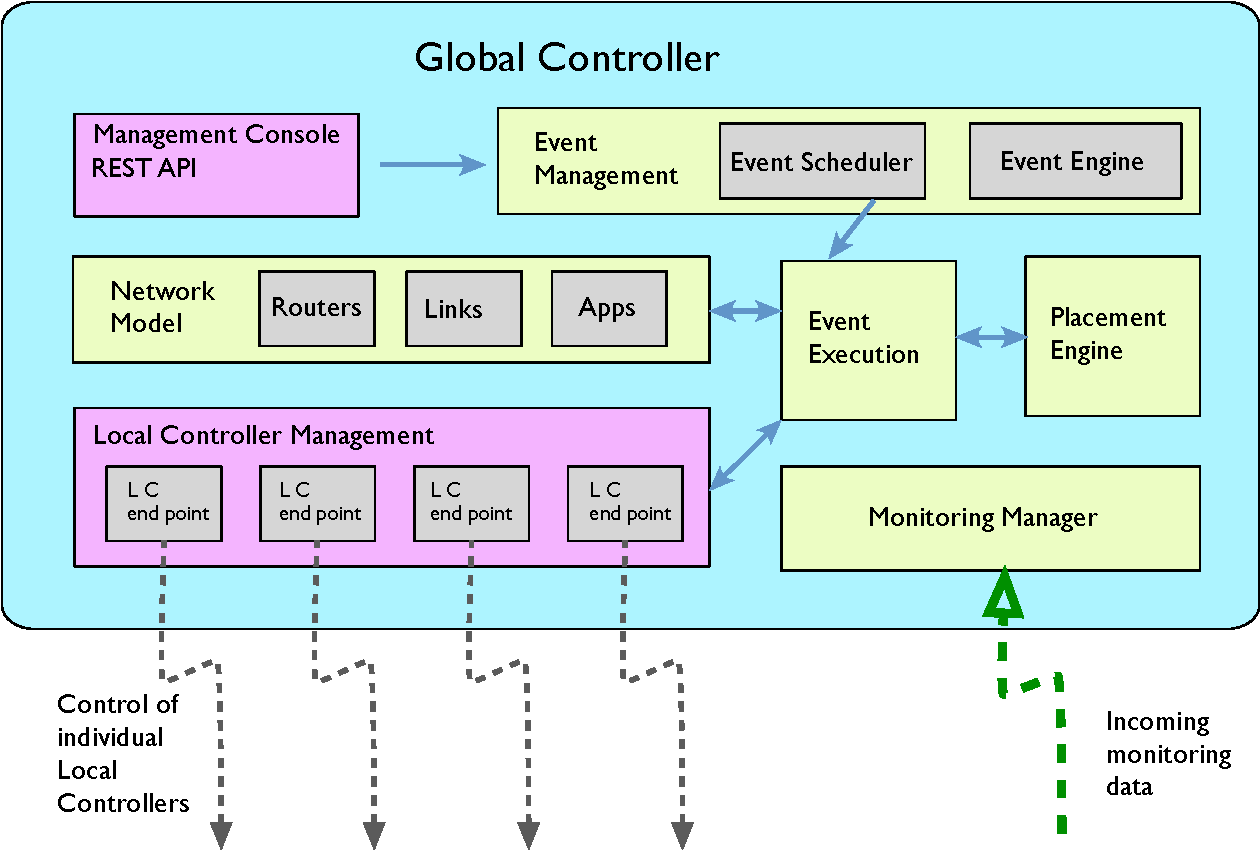
\includegraphics[width=14.5cm]{images/global_controller}
    \caption{Global Controller Architecture}
    \label{global-controller}
\end{figure}

The main elements of the Global Controller are:

\begin{description}[leftmargin=1.5em,labelindent=0,itemsep=3pt]

\item \textit{Event Management:} This is responsible for the runtime operation,
including support for event-based notifications and time scheduling of
events.  All setups that use the Probabilistic Experiment Control will
use an $Event Engine$ that generates events for router creation, link
creation, and router deletion.  These events are queued for
future activation in an $Event Scheduler$.  The configuration files
specify which probability distributions are used for these operations.

For setups using the REST API for Dynamic Programmable Control, the
call to the Management Console is converted into an event that
executes immediately.

\item \textit{Management Console - REST API:} This is an HTTP listener
  that supports the REST API into the Global Controller, and essentially the whole
  of VLSP.

\item \textit{Event Execution:} This executes the actions for each of
the events that the  $Event Scheduler$ chooses as the next action.
Each Event has a time, an event type, and some event
parameters. During event execution there is a handler for each type of
event, which causes the relevant actions to be performed.

\item \textit{Placement Engine:} This decides where to place a new
  router when one is created. The Placement Engine uses data about the
  current state, context, and configuration of the system to choose a
  location. The Placement Engine is a flexible part of VLSP and can be
  changed at run-time under software control.

\item \textit{Network Model:} This keeps information on the topology
  of the virtual network that has been created and is being managed,
  including all of the $Routers$ and $Links$. It also contains
  information on the $Apps$ that are running on eahc virtual router.
  The Model is used by many components in the Global Controller for
  decision making, outputs via the REST API, as well as visualization.

\item \textit{Monitoring Manager:} This manages the monitoring
  sub-system of VLSP.  It starts any configured probes on the virtual
  routers, and starts any configured data consumers and data reporters. The monitoring
  data is used by many components inside the Global Controller.

\item \textit{Local Controller Management:}  This is responsible for
  starting Local Controllers on specified hosts, interacting directly
  with those Local Controllers, and managing their state.  This
  element has an $end-point$ for each Local Controller that has been
  defined, as well as a direct network connection to that Local
  Controller for sendign it commands.

  All operations to start and stop routers, and commands for routers
  are directed through the relevant Local Controller.

  
\end{description}


\subsubsection{Management Console}

The Management Console supports the REST API into the Global
Controller.
All of the REST commands are presented in Appendix \ref{chap:restapi}.

\subsubsection{Placement Engine}

We have experimented with various placement algorithms, more details
of which can be found in our other papers. The \emph{Placement
Engine} of VLSP is the management component in charge of performing the
actual placement of the virtual entities and the application nodes
they host, according to the initial topology and the resource usage of
the virtual network elements. This is an important feature because,
when we configure a network or a service, given initial context
information, some of these parameters may change during the course of
the system’s operation and a reconfiguration may be required to
maintain optimized behaviour. Consequently, our approach has a
mechanism to achieve adaptation in a flexible manner.

The decision of the \emph{Placement Engine}, which can be changed at
run-time under software control, is encoded in an algorithm which can
be either rather simple, such as counting the number of virtual
routers on a host, or it can be complex, based on a set of constraints
and policies that represent the network properties. Therefore, to
determine the placement for the ‘next’ virtual router, the
GlobalController uses the defined Placement Engine.

The name of the Placement Engine class is set in the
\texttt{<PlacementEngineClass>} field.
The default class name is: \texttt{usr.globalcontroller.LeastUsedLoadBalancer}.
This is a list of the current implementations:

\begin{adjustwidth}{\parindent}{} % was 2em but \parindent is better
\begin{verbatim}
usr.globalcontroller.LeastBusyPlacement
usr.globalcontroller.LeastUsedLoadBalancer
usr.globalcontroller.NupPlacement
usr.globalcontroller.EnergyEfficientPlacement
\end{verbatim}
\end{adjustwidth}


\noindent The user can write their own Placement Engine, and set it in the
config  Such a Placement Engine can take into account any attributes
that are needed to make a decision 
which chooses a particular Local Controller.

\subsubsection{Monitoring Manager}

The Monitoring Manager is responsible for starting, stopping, and
processing the monitoring processes within VLSP.
Probes can be configured to start in the Routers which send various
kinds of measurment data related to different router processes and
tasks.

\subsubsection*{Router Probes}

The current set of probes that have been defined are:


{
  \small

  \begin{longtable}{ | p{5.7cm} | p{8.7cm} | }

\hline
\textbf{Name} & \textbf{Description} \\
\hline
\texttt{usr.router.AppListProbe} & This probe sends a list of all the executing
applications in a router. \newline
% /tmp/gc-channel10.out
The probe sends the \texttt{RouterName} plus
a table of \texttt{Data} with 1 row per app.

\vspace{\baselineskip}
\begin{tabular}{ p{8.3cm} }
  \hline
  ProbeAttributeType.STRING \\
  \hline
  \texttt{RouterName} \\
  \hline
  TableProbeAttribute \\
  \hline
  \texttt{Data} \\
  \hline 
\begin{lstlisting}[language=java] 
"AID", ProbeAttributeType.INTEGER
"StartTime", ProbeAttributeType.LONG
"ElapsedTime", ProbeAttributeType.LONG
"RunTime", ProbeAttributeType.LONG
"UserTime", ProbeAttributeType.LONG
"SysTime", ProbeAttributeType.LONG
"State", ProbeAttributeType.STRING
"ClassName", ProbeAttributeType.STRING
"Args", ProbeAttributeType.STRING
"Name", ProbeAttributeType.STRING
"RuntimeKeys", ProbeAttributeType.LIST
"RuntimeValues", ProbeAttributeType.LIST
\end{lstlisting} \\
  \hline
\end{tabular}

\\
\hline
\texttt{usr.router.NetIFStatsProbe} & This probe sends a list of stats
for each of the network interfaces of the Router. \newline
% /tmp/gc-channel7.out 
The probe sends the \texttt{RouterName} plus
a table of \texttt{Data} with 1 row per app.

\vspace{\baselineskip}
\begin{tabular}{ p{8.3cm} }
  \hline
  ProbeAttributeType.STRING \\
  \hline
  \texttt{RouterName} \\
  \hline
  TableProbeAttribute \\
  \hline
  \texttt{Data} \\
  \hline
\begin{lstlisting}[language=java]
"name", ProbeAttributeType.STRING
"InBytes", ProbeAttributeType.INTEGER
"InPackets", ProbeAttributeType.INTEGER
"InErrors", ProbeAttributeType.INTEGER
"InDropped", ProbeAttributeType.INTEGER
"InDataBytes", ProbeAttributeType.INTEGER
"InDataPackets", ProbeAttributeType.INTEGER
"OutBytes", ProbeAttributeType.INTEGER
"OutPackets", ProbeAttributeType.INTEGER
"OutErrors", ProbeAttributeType.INTEGER
"OutDropped", ProbeAttributeType.INTEGER
"OutDataBytes", ProbeAttributeType.INTEGER
"OutDataPackets", ProbeAttributeType.INTEGER
"InQueue", ProbeAttributeType.INTEGER
"BiggestInQueue", ProbeAttributeType.INTEGER
"OutQueue", ProbeAttributeType.INTEGER
"BiggestOutQueue", ProbeAttributeType.INTEGER
\end{lstlisting} \\
\hline
\end{tabular}

\\
\hline
\texttt{usr.router.ThreadGroupListProbe} & This probe sends data for
each Thread Group in the Router.  \newline
%/tmp/gc-channel14.out
The probe sends the \texttt{RouterName} plus
a table of \texttt{Data} with 1 row per app.

\vspace{\baselineskip}
\begin{tabular}{ p{8.3cm} }
  \hline
  ProbeAttributeType.STRING \\
  \hline
  \texttt{RouterName} \\
  \hline
  TableProbeAttribute \\
  \hline
  \texttt{Data} \\
  \hline
\begin{lstlisting}[language=java]
"Name", ProbeAttributeType.STRING
"StartTime", ProbeAttributeType.LONG
"ElapsedTime", ProbeAttributeType.LONG
"RunTime", ProbeAttributeType.LONG
"UserTime", ProbeAttributeType.LONG
"SysTime", ProbeAttributeType.LONG
"Mem", ProbeAttributeType.LONG
\end{lstlisting} \\
\hline
\end{tabular}

\\
\hline
\texttt{usr.router.ThreadListProbe} & This probe sends data for
each Thread Group in the Router.  \newline
% /tmp/gc-channel15.out
The probe sends the \texttt{RouterName} plus
a table of \texttt{Data} with 1 row per app.


\vspace{\baselineskip}
\begin{tabular}{ p{8.3cm} }
  \hline
  ProbeAttributeType.STRING \\
  \hline
  \texttt{RouterName} \\
  \hline
  TableProbeAttribute \\
  \hline
  \texttt{Data} \\
  \hline
\begin{lstlisting}[language=java]
"Name", ProbeAttributeType.STRING
"StartTime", ProbeAttributeType.LONG
"ElapsedTime", ProbeAttributeType.LONG
"RunTime", ProbeAttributeType.LONG
"UserTime", ProbeAttributeType.LONG
"SysTime", ProbeAttributeType.LONG
"Mem", ProbeAttributeType.LONG
"ThreadGroup", ProbeAttributeType.STRING
\end{lstlisting} \\
\hline
\end{tabular}

\\
\hline
\end{longtable}


\normalsize
}


\subsubsection*{Local Controller Probe}

There is currently one probe residing in the Local Controller.
It is turned on automatically if monitoring is configured to be on.
This probe is designed to send host based info back to the Global
Controller. 


{
  \small

  \begin{longtable}{ | p{5.7cm} | p{8.7cm} | }

\hline
\textbf{Name} & \textbf{Description} \\
\hline
\texttt{usr.localcontroller. HostInfoProbe} & This probe sends data
about the physical host that the LocalController is managing. \newline
% /tmp/gc-channel13.out
The probe sends the \texttt{Name} of the host, cpu usage, memory usage,
plus a table of network statistics, with 1 row per network interface
of the physical host.

\vspace{\baselineskip}
\begin{tabular}{ p{8.3cm} }
  \hline
  ProbeAttributeType.STRING \\
  \hline
  \texttt{Name} \\
  \hline
  ProbeAttributeType.FLOAT \\
  \hline
  \texttt{cpu-user} \\
  \hline
  ProbeAttributeType.FLOAT \\
  \hline
  \texttt{cpu-sys} \\
  \hline
  ProbeAttributeType.FLOAT \\
  \hline
  \texttt{cpu-idle} \\
  \hline
  ProbeAttributeType.FLOAT \\
  \hline
  \texttt{load-average} \\
  \hline
  ProbeAttributeType.INTEGER \\
  \hline
  \texttt{mem-used} \\
  \hline
  ProbeAttributeType.INTEGER \\
  \hline
  \texttt{mem-free} \\
  \hline
  ProbeAttributeType.INTEGER \\
  \hline
  \texttt{mem-total} \\
  \hline
  TableProbeAttribute \\
  \hline
  \texttt{net-stats} \\
  \hline
\begin{lstlisting}[language=java]
"if-name", ProbeAttributeType.STRING
"in-packets", ProbeAttributeType.LONG
"in-bytes", ProbeAttributeType.LONG
"out-packets", ProbeAttributeType.LONG
"out-bytes", ProbeAttributeType.LONG
\end{lstlisting} \\
  \hline
\end{tabular}

\\
\hline
  \end{longtable}

 
\normalsize
}

\subsubsection*{Global Controller Reporters}

The reporters which can be configured in the Global Controller are
designed to collect measurements which are sent by the probes in other
parts of the system.


The current set of probes that have been defined are:


{
  \small

  \begin{longtable}{ | p{5.7cm} | p{8.7cm} | }

\hline
\textbf{Name} & \textbf{Description} \\
\hline
\texttt{usr.globalcontroller. HostInfoReporter} & This reporter
collects measurements from the \texttt{HostInfoProbe} embedded in the
Local Controller.

Additionally data is sent to /tmp/gc-channel13.out.
\hline
\texttt{usr.globalcontroller. RouterAppsReporter} & This reporter
collects measurements from the \texttt{AppListProbe} embedded in the
router, if it has been configured.

Additionally data is sent to /tmp/gc-channel10.out.
\hline
\texttt{usr.globalcontroller. NetIFStatsReporter} & This reporter
collects measurements from the \texttt{NetIFStatsProbe} embedded in the
router, if it has been configured.

Additionally data is sent to /tmp/gc-channel7.out.
\hline
\texttt{usr.globalcontroller. ThreadGroupListReporter} & This reporter
collects measurements from the \texttt{ThreadGroupListProbe} embedded in the
router, if it has been configured.

Additionally data is sent to /tmp/gc-channel14.out.
\hline
\texttt{usr.globalcontroller. ThreadListReporter} & This reporter
collects measurements from the \texttt{ThreadListProbe} embedded in the
router, if it has been configured.

Additionally data is sent to /tmp/gc-channel15.out.
\hline
  \end{longtable}

 
\normalsize
}


\subsection{The Local Controller}

The Local Controller is a per host Host Controller that accepts
commands that are specifically for that host.
The Local Controller acts as a management point for starting and
stopping Routers, for creating and deleting links, and also for
monitoring the host it runs on.

\subsection{Routers}

The Routers themselves have multiple network interfaces, one interface
for each connection to another router, as well as 6 internal main
functional blocks.

\begin{figure}[h!]
    \centering
    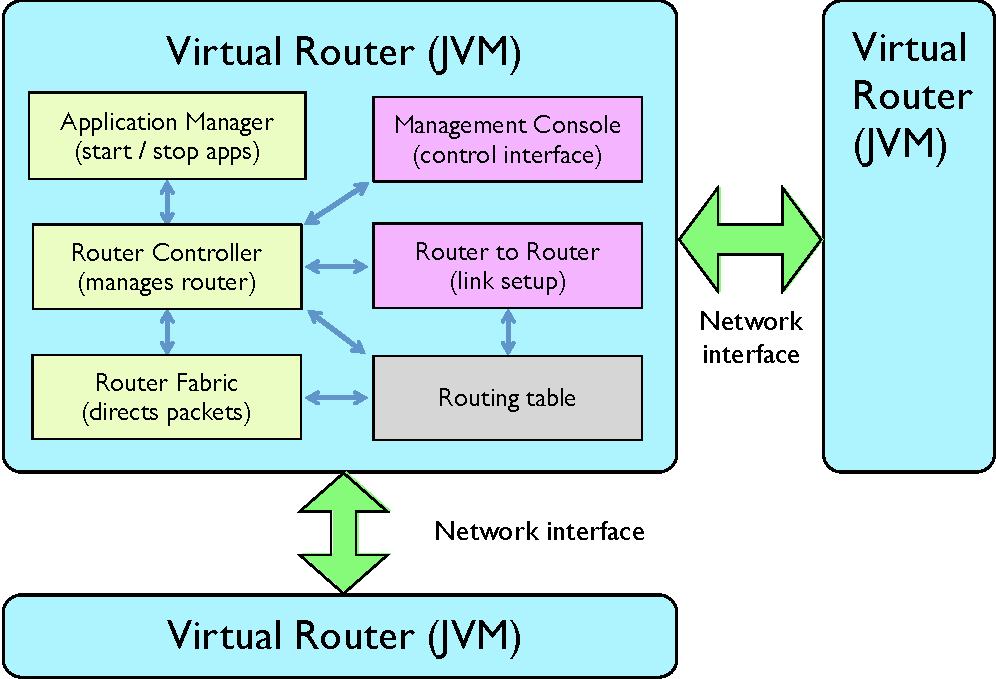
\includegraphics[width=11cm]{images/router-main-blocks}
    \caption{Router Top Level View with Main Functional Blocks}
    \label{design:router-main-blocks}
\end{figure}





The Router functions include:

\begin{itemize}

\item \emph{Management Console} -- which provides a control interface from the
  outside world

\item \emph{Router to Router} -- which provides the mechanism to setup new
  connections to other routers

\item \emph{Router Controller} -- which controls the internal operation of
  the router

\item \emph{Router Fabric} -- which connects the network interfaces to
  the router and provides the forwarding mechanism

\item \emph{Routing Table} -- which holds information about how to
  route datagrams

\item \emph{Application Manager} -- which starts up and shuts down
  applications that might run on the router

\end{itemize}

\noindent Each of these is shown in figure \ref{design:router-main-blocks}.



Each of the functional blocks is manifested into an design
element within the interal architecture of the router.


\begin{figure}[h!]
    \centering
    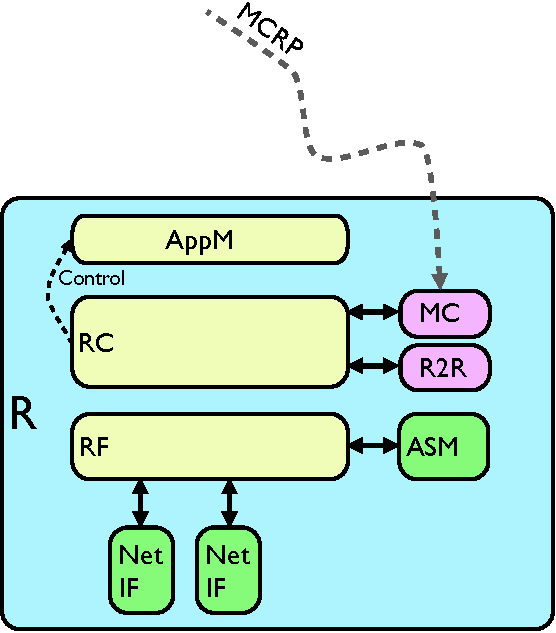
\includegraphics[width=7cm]{images/router-elements}
    \caption{Router Internal Architecture}
    \label{design:router-elements}
\end{figure}


These functions include:

\begin{itemize}

\item \emph{MC} -- Management Consolewhich provides a control interface from the
  outside world

\item \emph{R2R} -- Router to Router which provides the mechanism to setup new
  connections to other routers

\item \emph{RC} -- Router Controller which controls the internal operation of
  the router

\item \emph{RF} -- Router Fabric which connects the network interfaces to
  the router and provides the forwarding mechanism

\item \emph{AppM} -- Application Manager which starts up and shuts down
  applications that might run on the router

\item \emph{NetIF} -- a Network Interface to another virtual Router.

\item \emph{ASM} -- the Application Socket Mux - which is the Network
  Interface to the local router. All \emph{Sockets} for local apps are
  multiplexed through this interface.

\end{itemize}

\noindent Each of these is shown in figure \ref{design:router-elements}.



\subsubsection{Connecting Routers}

In this section the mechanism by whch one Router connects to another
Router in order to create a new virtual network connection is shown.

Each virtual router is connected directly to another virtual router
via a Network Interface (NetIF).
The connection can be configured to be a TCP connection or a UDP
connection.

The TCP connection gives an underlying transport for the traffic that
is reliable. 

The UDP connection gives an underlying transport for the traffic that
is unreliable.

In figure \ref{design:two-routers}, two apps are started on a Router,
each with it's own Socket.  We see how the Socket is connected to the
Router Fabric via the ASM.

\begin{figure}[h!]
    \centering
    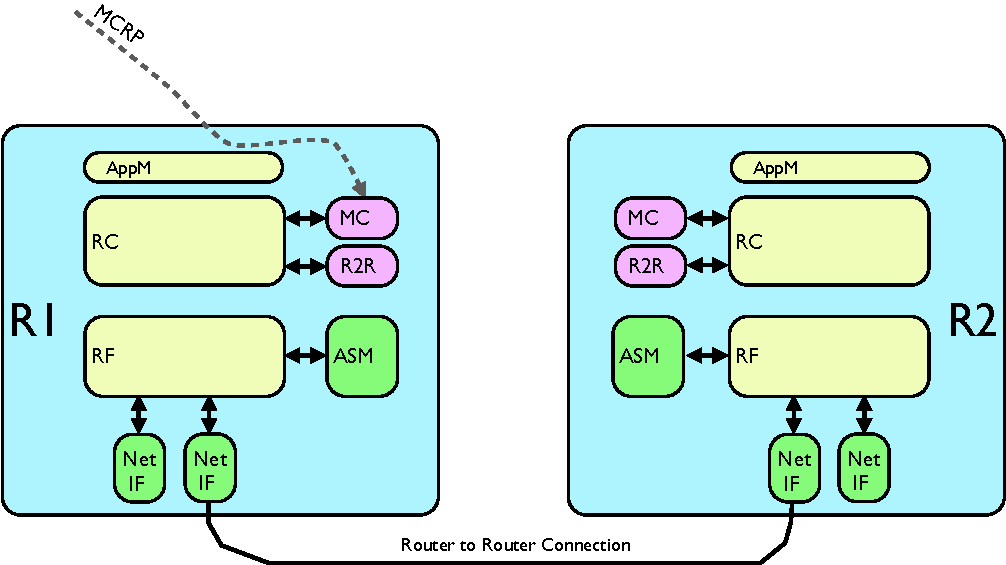
\includegraphics[width=12cm]{images/two-routers}
    \caption{Two Routers}
    \label{design:two-routers}
\end{figure}

\subsubsection{Applications and Application Lifecycle}

Applications and services on the platform are run as applications on a router.

Each router has a local network interface that provides a Socket level
API for these applications.  In appendix \ref{chap:methods}, there is
are full details of this API.

This Socket level API presents a UDP-like socket that can be used for
writing networking applications that run directly on the router.
These applications are started at run-time by making a call to the
Global Controller, passing in the name of the class and the arguments
it needs to start up.


\begin{figure}[h!]
    \centering
    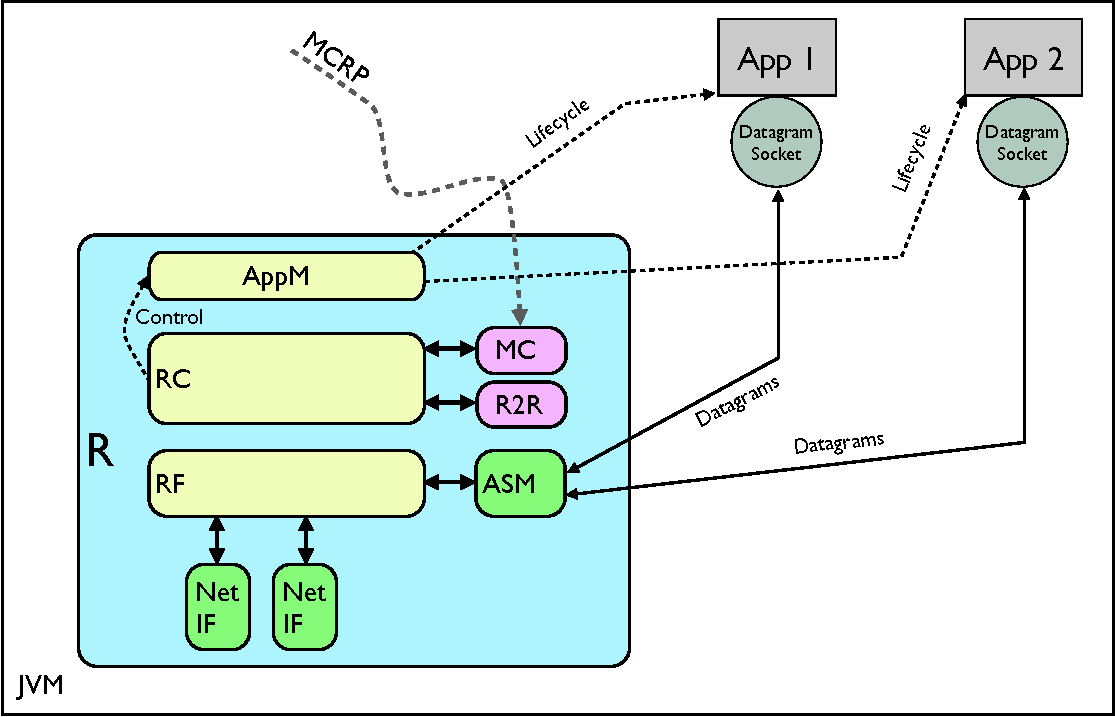
\includegraphics[width=11cm]{images/app-manager}
    \caption{Application Manager and Application Lifecycle}
    \label{design:app-manager}
\end{figure}





\section{System Programmability}
\label{chap:programmability}
\subsection{Writing Applications and Services}

All applications are started under control of the Application Manager
and must implement the  Java interface \texttt{usr.applications.Application}.

\begin{lstlisting}[language=java,frame=single]
/**
 * An Application has is a Runnable object that has a managed lifecycle.
 */
public interface Application extends Runnable {
    /**
     * Initialize with some args
     */
    public ApplicationResponse init(String[] args);

    /**
     * Start an application. This is called before run().
     */
    public ApplicationResponse start();

    /**
     * Stop an application.
     * This is called to implement graceful shut down and cause run() to end.
     */
    public ApplicationResponse stop();
}
\end{lstlisting}

\noindent Notice that \texttt{Application} extends \texttt{Runnable},
so this means that applications must have a \texttt{run()} method.
This is where the \emph{main} body of the app resides.

The ApplicationResponse object has 2 fields: (i) a $boolean$
value to indicate if the app is progressing well, where $true$ means
success and $false$ mean failure, (ii) a message that may be passed
on.

If any of these methods returns an ApplicationResponse with a
$false$ value then the system will stop what it is doing, and clean up
the application context.

\subsubsection{An Example App -- Sending Data}

Here is an app that opens a Socket and sends datagrams.
When it is started it takes 3 arguments: an address to send to, a port
to send to, and a count of the number of datagrams.

\begin{lstlisting}[language=java,frame=single]
public class Send implements Application {
    Address addr = null;
    int port = 0;
    int count = 0;

    boolean running = false;
    DatagramSocket socket = null;
    
\end{lstlisting}


\noindent  The \texttt{init()} method is defined to process all the
arguments that are passed in.

\begin{lstlisting}[language=java,frame=single]
    public ApplicationResponse init(String[] args) {
        if (args.length == 3) {
            // try address
            try {
                addr = AddressFactory.newAddress(args[0]);

            } catch (Exception e) {
                return new ApplicationResponse(false, "UnknownHost " + args[0]);
            }

            // try port
            Scanner scanner = new Scanner(args[1]);

            if (scanner.hasNextInt()) {
                port = scanner.nextInt();
                scanner.close();
            } else {
            	scanner.close();
                return new ApplicationResponse(false, "Bad port " + args[1]);
            }

            // try count
            scanner = new Scanner(args[2]);

            if (scanner.hasNextInt()) {
                count = scanner.nextInt();
                scanner.close();
            } else {
            	scanner.close();
                return new ApplicationResponse(false, "Bad count " + args[2]);
            }

            // we got here ok so return true
            return new ApplicationResponse(true, "");

        } else {
            return new ApplicationResponse(false, "Usage: Send address port count");
        }
    }
\end{lstlisting}

\noindent If the application returns an ApplicationResponse with a
$true$ value then the system will progress to the \texttt{start()}
method.

In this case the application creates a new socket and connects to the
remote router. If the connect fails then the ApplicationResponse is
$false$ and the application will stop, otherwise it returns an
ApplicationResponse with $true$ and it progresses to the
\texttt{run()} method.

\begin{lstlisting}[language=java,frame=single]
    public ApplicationResponse start() {
        try {
            // set up socket
            socket = new DatagramSocket();

            socket.connect(addr, port);

        } catch (Exception e) {
            return new ApplicationResponse(false, "Cannot open socket " + e.getMessage());
        }

        running = true;

        return new ApplicationResponse(true, "");
    }
\end{lstlisting}

\noindent The \texttt{run()} method creates a new datagram and sends
it onwards.

\begin{lstlisting}[language=java,frame=single]
    public void run() {
        Datagram datagram = null;

        // a buffer for data
        byte [] buffer;

        // loop around        
        for (int i = 0; i < count; i++) {
            // Code to Fill the Buffer

            datagram = DatagramFactory.newDatagram(buffer);

            try {
                socket.send(datagram);

            } catch (Exception e) {
                if (socket.isClosed()) {
                    break;
                } else {
                    // maybe try again
                }
            }
        }
    }
\end{lstlisting}

\noindent Finally the \texttt{stop()} method is shown.
This method is called by the Application Manager when the Application
is terminated in some way, either by explicitly being stopped by a
REST API call or by shutting down the whole system.


\begin{lstlisting}[language=java,frame=single]
    public ApplicationResponse stop() {
        running = false;

        if (socket != null) {
            socket.close();
        }

        return new ApplicationResponse(true, "");
    }
\end{lstlisting}

\subsubsection{An Example App -- Receiving Data}

Here is an app that opens a Socket and receives datagrams.
When it is started it takes 1 argument, whic is the port to listen on.

\begin{lstlisting}[language=java,frame=single]
public class Recv implements Application {
    int port = 0;

    int count = 0;

    boolean running = false;
    DatagramSocket socket = null;

\end{lstlisting}

\noindent  The \texttt{init()} method is defined to process the
arguments that are passed in.

\begin{lstlisting}[language=java,frame=single]
    public ApplicationResponse init(String[] args) {
        if (args.length == 1) {
            // try port
            Scanner scanner = new Scanner(args[0]);

            if (scanner.hasNextInt()) {
                port = scanner.nextInt();
                scanner.close();
            } else {
            	scanner.close();
                return new ApplicationResponse(false, "Bad port " + args[1]);
            }

            return new ApplicationResponse(true, "");

        } else {
            return new ApplicationResponse(false, "Usage: Recv port");
        }
    }
    
\end{lstlisting}


\noindent Again, if the application returns an ApplicationResponse with a
$true$ value then the system will progress to the \texttt{start()}
method.

In this case the application creates a new socket and
$binds$ to the specified port.
If this fails then the ApplicationResponse is
$false$ and the application will stop, otherwise it returns an
ApplicationResponse with $true$ and it progresses to the
\texttt{run()} method.

\begin{lstlisting}[language=java,frame=single]
    public ApplicationResponse start() {
        try {
            // set up socket
            socket = new DatagramSocket();

            socket.bind(port);

        } catch (Exception e) {
            return new ApplicationResponse(false, "Cannot open socket " + e.getMessage());
        }

        running = true;

        return new ApplicationResponse(true, "");
    }

\end{lstlisting}


\noindent The \texttt{run()} method receives each datagram 
prints out some meta-data.

\begin{lstlisting}[language=java,frame=single]
    public void run() {
        Datagram datagram;

        try {
            while ((datagram = socket.receive()) != null) {

                System.out.print(count + ". ");
                System.out.print("HdrLen: " + datagram.getHeaderLength() +
                                 " Len: " + datagram.getTotalLength() +
                                 " Time: " + (System.currentTimeMillis() - 
                                                    datagram.getTimestamp()) +
                                 " From: " + datagram.getSrcAddress() +
                                 " To: " + datagram.getDstAddress() +
                                 ". ");

                byte[] payload = datagram.getPayload();

                if (payload == null) {
                    System.out.print("No payload");
                } else {
                    System.out.print(new String(payload));
                }
                System.out.println("");

                count++;
            }
        } catch (SocketException se) {
            System.out.println(se.getMessage());
        }
    }
    
\end{lstlisting}

\noindent Finally the \texttt{stop()} method is shown.
This method is called by the Application Manager when the Application
is terminated in some way, either by explicitly being stopped by a
REST API call or by shutting down the whole system.

\begin{lstlisting}[language=java,frame=single]
    public ApplicationResponse stop() {
        running = false;

        if (socket != null) {
            socket.close();
        }

        return new ApplicationResponse(true, "");
    }
\end{lstlisting}

\subsection{Writing Topology and Management Applications}

This section presents the ways of writing topology focused
applications and management
applications for VLSP.  Such applications can include scenarios such
as: (i) experiment setup, control, and execution; (ii) orchestration
strategies; (iii) dashboards; etc.




\subsubsection{VIM Client}

The Vim Client, \texttt{usr.vim.VimClient} is a Java wrapper
for the REST API, detailed in appendix \ref{chap:restapi}.
The VimClient methods are shown in detail in appendix \ref{chap:vimclient},
It is possible to write a Vim Client in any language, and we have
versions of them written in \texttt{clojure},  \texttt{Julia} and also
 \texttt{python}.

If you do not have VLSP Client yet, you can find the source on
\textit{gitlab} at

\code{https://gitlab.com/sclayman/vlsp-client}

 


In the following example we show how to use the VimClient to create a
virtual network.

\begin{figure}[ht!]
  \centering
  \resizebox{0.7\textwidth}{!}{%

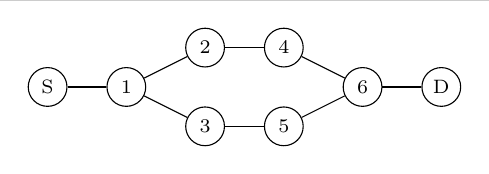
\begin{tikzpicture}%
  \node[circle,draw=black, fill=none, inner sep=0pt,
    minimum size=14pt, font=\scriptsize] (r1) at (1,0.5) {1};
      
  \node[circle,draw=black, fill=none, inner sep=0pt, 
    minimum size=14pt, font=\scriptsize]  (r2) at (2,1) {2};
  
  \node[circle,draw=black, fill=none, inner sep=0pt,
    minimum size=14pt, font=\scriptsize] (r3) at (2,0) {3};

  \node[circle,draw=black, fill=none,  inner sep=0pt,
    minimum size=14pt, font=\scriptsize] (r4) at (3,1) {4};

  \node[circle,draw=black, fill=none, inner sep=0pt,
    minimum size=14pt, font=\scriptsize] (r5) at (3,0) {5};

  \node[circle,draw=black, fill=none,  inner sep=0pt,
    minimum size=14pt, font=\scriptsize] (r6) at (4,0.5) {6};

  \node[circle,draw=black, fill=none,  inner sep=0pt,
    minimum size=14pt, font=\scriptsize] (rS) at (0,0.5) {S};

  \node[circle,draw=black, fill=none,  inner sep=0pt,
    minimum size=14pt, font=\scriptsize] (rD) at (5,0.5) {D};

      \draw [-] (r1) -- (r2);
      \draw [-] (r1) -- (r3);
      \draw [-] (r2) -- (r4);
      \draw [-] (r3) -- (r5);
      \draw [-] (r4) -- (r6);
      \draw [-] (r5) -- (r6);
      \draw [-] (rS) -- (r1);
      \draw [-] (r6) -- (rD);
    \end{tikzpicture}
}

\caption{Network - 8 Nodes}
  \label{fig:8nodes}
\end{figure}


\noindent First, a new VimClient is created with a connection to the
$GlobalController$.  The name of the host running the GlobalController
is specified, as well as the port it is listening on.

\begin{lstlisting}[language=Java,frame=single]
    VimClient conn = new VimClient($gc\_host$, 8888);

\end{lstlisting}

\noindent Then the virtual routers are created.  Each call to
\texttt{createRouter()} will create a new router, and return a JSON
value.  The return values are described in Appendix \ref{chap:restapi}
- the REST API Component Interaction.

\begin{lstlisting}[language=Java,frame=single]
    JSONObject r1 = conn.createRouter();
    int router1 = (Integer)r1.get("routerID");

    JSONObject r2 = conn.createRouter();
    int router2 = (Integer)r2.get("routerID");

    JSONObject r3 = conn.createRouter();
    int router3 = (Integer)r3.get("routerID");

    JSONObject r4 = conn.createRouter();
    int router4 = (Integer)r4.get("routerID");

    JSONObject r5 = conn.createRouter();
    int router5 = (Integer)r5.get("routerID");

    JSONObject r6 = conn.createRouter();
    int router6 = (Integer)r6.get("routerID");

    JSONObject rS = conn.createRouter();
    int routerS = (Integer)rS.get("routerID");

    JSONObject rD = conn.createRouter();
    int routerD = (Integer)rD.get("routerID");

\end{lstlisting}

\noindent Then the links are created between the virtual routers.

\begin{lstlisting}[language=Java,frame=single]
    JSONObject l1 = conn.createLink(router1, router2, 10);
    int link1 = (Integer)l1.get("linkID");

    JSONObject l2 = conn.createLink(router1, router3, 10);
    int link2 = (Integer)l2.get("linkID");

    JSONObject l3 = conn.createLink(router2, router4, 10);
    int link3 = (Integer)l3.get("linkID");

    JSONObject l4 = conn.createLink(router3, router5, 10);
    int link4 = (Integer)l4.get("linkID");

    JSONObject l5 = conn.createLink(router4, router6, 10);
    int link5 = (Integer)l5.get("linkID");

    JSONObject l6 = conn.createLink(router5, router6, 10);
    int link6 = (Integer)l6.get("linkID");

    JSONObject lSto1 = conn.createLink(routerS, router1, 10);
    int linkSto1 = (Integer)lSto1.get("linkID");

    JSONObject lDto6 = conn.createLink(routerD, router6, 10);
    int linkDtoS = (Integer)lDto6.get("linkID");
\end{lstlisting}


\subsection{Extending The VIM}

The Virtual Infrastructure Manager (VIM) is the Global Controller in
VLSP.
It has been designed to be adaptable and extendtable for various
needs. It implements a class called: $Lifecycle$.

\begin{lstlisting}[language=java]
  public class MyVim extends GlobalController {
    ....
  }

\end{lstlisting}

\noindent There are 3 main lifecycle methods:

\noindent Init the VIM
\begin{lstlisting}[language=Java]
    $\rhd$ public boolean init();
\end{lstlisting}

\noindent Start the VIM
\begin{lstlisting}[language=Java]
    $\rhd$ public boolean start();
\end{lstlisting}

\noindent Stop the VIM
\begin{lstlisting}[language=Java]
    $\rhd$ public boolean stop();
\end{lstlisting}



\subsubsection{GlobalController Hooks}

Also there are a set of hooks / callback functions that have
been embedded in the Global Controller that can be called in
subclasses to allow flexible operation on top of the normal behaviour
of the Global Controller.


\noindent This is called at then end of init phase.
\begin{lstlisting}[language=Java]
    $\rhd$ public boolean postInitHook();
\end{lstlisting}

\noindent This is called at then beginning of the start phase.
\begin{lstlisting}[language=Java]
    $\rhd$ public boolean preStartHook();
\end{lstlisting}

\noindent This is called at then end of the start phase.
\begin{lstlisting}[language=Java]
    $\rhd$ public boolean postStartHook();
\end{lstlisting}

\noindent This is called at then beginning of the stop phase.
\begin{lstlisting}[language=Java]
    $\rhd$ public boolean preStopHook();
\end{lstlisting}

\noindent This is called at then end of the stop phase.
\begin{lstlisting}[language=Java]
    $\rhd$ public boolean postStopHook();
\end{lstlisting}

\noindent This is called at regular intervals during normal execution.
\begin{lstlisting}[language=Java]
    $\rhd$ public boolean runLoopHook();
\end{lstlisting}

\noindent This is called at then beginning of the shutting down the system.
\begin{lstlisting}[language=Java]
    $\rhd$ public boolean preShutdownHook();
\end{lstlisting}

\noindent This is called at then end of the shutting down the
system. It is nearly the last operation. 
\begin{lstlisting}[language=Java]
    $\rhd$ public boolean postShutdownHook();
\end{lstlisting}

\noindent This is called just after a router is started.
\begin{lstlisting}[language=Java]
     $\rhd$ public boolean routerStartedHook(int id);
\end{lstlisting}

\noindent This is called just after a router is stopped.
\begin{lstlisting}[language=Java]
    $\rhd$ public boolean routerEndedHook(int id);
\end{lstlisting}

\noindent This is called at then just before a LocalController is started.
\begin{lstlisting}[language=Java]
    $\rhd$ public boolean preLocalControllerStartHook(LocalControllerInfo lcInfo);
\end{lstlisting}

\noindent This is called at then just after a LocalController is started.
\begin{lstlisting}[language=Java]
    $\rhd$ public boolean postLocalControllerStartHook(LocalControllerInfo lcInfo);
\end{lstlisting}

\noindent This is called at then just before a LocalController is stopped.
\begin{lstlisting}[language=Java]
    $\rhd$ public boolean preLocalControllerStopHook(LocalControllerInfo lcInfo);
\end{lstlisting}

\noindent This is called at then just after a LocalController is stopped.
\begin{lstlisting}[language=Java]
    $\rhd$ public boolean postLocalControllerStopHook(LocalControllerInfo lcInfo);
\end{lstlisting}



\subsubsection{Writing A Placement Engine}

As stated earlier, the \emph{Placement
Engine} of VLSP is the management component in charge of performing the
actual placement of the virtual entities and the application nodes
they host, according to the initial topology and the resource usage of
the virtual network elements.
The system already comes with the following Placement Engines:

\begin{adjustwidth}{\parindent}{} % was 2em but \parindent is better
\begin{verbatim}
usr.globalcontroller.LeastBusyPlacement
usr.globalcontroller.LeastUsedLoadBalancer
usr.globalcontroller.NupPlacement
usr.globalcontroller.EnergyEfficientPlacement
\end{verbatim}
\end{adjustwidth}

\begin{sloppypar}
\noindent  All Placement Engines classes need to implement this Java interface:
\texttt{usr.globalcontroller.PlacementEngine} which shown here:
\end{sloppypar}


\begin{lstlisting}[language=Java,frame=single]
  /**
 * A PlacementEngine is repsonsible for determining the placement
 * of a Router across the active resources.
 */
public interface PlacementEngine {

    /**
     * Get the relevant LocalControllerInfo for a placement of a router with 
     * a specified name and address.
     */
    public LocalControllerInfo routerPlacement(String name, String address);

    /**
     * Get the relevant LocalControllerInfo for a placement of a router with 
     * a specified name and address, but also supplying extra parameters. It 
     * is used for prediction of future load.
     */
    public LocalControllerInfo routerPlacement(String name, String address,
                                                    String parameters);
    
    /**
     * Get all the possible placement destinations
     */
    public Set<LocalControllerInfo> getPlacementDestinations();
}
\end{lstlisting}


\noindent  Any time a new Router is created the router creation
mechanism will  eventually call into the GlobalController calling either this method:

\begin{lstlisting}[language=Java]
    /**
     * Do some placement calculation with extra parameter passing
     */
    public LocalControllerInfo placementForRouter(String name, String address) {
        return placementEngine.routerPlacement(name, address);
    }
\end{lstlisting}

\noindent or this method

\begin{lstlisting}[language=Java]
    /**
     * Do some placement calculation with extra parameter passing
     */
    public LocalControllerInfo placementForRouter(String name, String address,
                                                       String parameters) {
        return placementEngine.routerPlacement(name, address, parameters);
    }
\end{lstlisting}

\noindent depending on whether \emph{parameters} were passed in from
the outside.

Both of these methods  call directly into the PlacementEngine with a
name and address the system has chosen,  plus any parameters passed in
from the outside, if that option was called.
The value returned holds information about the nominated
LocalController for the actual placement.
Using this returned value, the GlobalController will actually start
the Router on that host. 


%% If you write your own PlacementEngine, you can grab this data, and
%% then choose a particular LocalController, based on your own
%% attributes. 



%\section{Summary}
%\label{chap:summary}
%
The benefits of the lightweight Integrated Virtual Platform which has
a virtual router and the
basic capabilities of a service component are:
\begin{itemize}
\item it provides a different way to do virtual networks: we can
  create arbitrary topologies using virtual routers 
\item uniform manageability of all types of virtual machines can be
  undertaken in the same environment
\item we can do more evaluations of service management functions by
  not using full VEEs and full services. For example, scalability can
  be evaluated more easily, and it can cover both 
  the dimension of virtual services as well as the dimension of
  virtual networks.
%\item we can do enhanced monitoring evaluations

\end{itemize}


\appendix{Appendix - Configuration Options}
\label{chap:config}
The following table presents the configuration options for the Global
Controller.

\subsection{Global Controller Configuration Options}

% The table of configuration options

\label{globalcontroller:config}

% This needs a few passes to layout correctly

{
  \renewcommand{\arraystretch}{1.6} 
  \renewcommand{\tabcolsep}{1.1ex}


\small

% longtable lines
\begin{longtable}{ | p{7.5cm} | p{6.5cm} | }

\caption{Global Controller Configuration Options} \\
  \hline \multicolumn{2}{| c |} {\textbf{Configuration Options}}\\
  \hline  {\textbf{Field}} & {\textbf{Description}} \\
\endhead




\hline
\footnotesize{\texttt{<SimOptions>} (required)} & The top level node for all
configuration options to the Global Controller. \\
\hline \hline

% GlobalController

\hline
\footnotesize{\texttt{<GlobalController>} (optional)} &
The node for specific options for  the Global Controller.  Only
one such section is allowed.
\\
\hline
\footnotesize{\texttt{<GlobalController> $\rightarrow$ <Simulation> (optional)}} &
If true, the Global Controller simulates routers rather than starting
them on local controllers.
\newline
Boolean, default is \texttt{false}. 
 \\
\hline
\footnotesize{\texttt{<GlobalController> $\rightarrow$ <Port> (optional)}} &
The port that the Global Controller should listen on. 
\newline
Integer value -- default is \texttt{8888}.
\\

\hline
\footnotesize{\texttt{<GlobalController> $\rightarrow$ <StartLocalControllers> (optional)}} &
Should the the Global Controller start any localcontrollers, if
necessary. 
\newline
Boolean, default is \texttt{true}.  If false GC assumes local controllers
started by hand.
 \\

\hline
\footnotesize{\texttt{<GlobalController> $\rightarrow$ <ConnectedNetwork> (optional)}} &
If true the GC will add a link to connect the network if it becomes
disconnected.
\newline
Boolean, default is \texttt{false}.
\\
\hline
\footnotesize{\texttt{<GlobalController> $\rightarrow$ <AllowIsolatedNodes> (optional)}} &
If false the GC will reconnect a node which has no links.
\newline
Boolean, default is \texttt{true}.
\\
\hline
\footnotesize{\texttt{<GlobalController> $\rightarrow$ <PlacementEngineClass> (optional)}} &
The name of the class of the placement engine in the Global Controller. 
\newline
String, default is \texttt{usr.globalcontroller. LeastUsedLoadBalancer}.
\\
\hline
\footnotesize{\texttt{<GlobalController> $\rightarrow$ <VisualizationClass> (optional)}} &
The name of the class for Visualization in the Global Controller. 
\newline
String, there is no default.
\\
\hline
\footnotesize{\texttt{<GlobalController> $\rightarrow$ <Monitoring> (optional)}} &
Should the Global Controller start the Lattice monitoring
framework on the routers. 
\newline
Boolean, default is \texttt{false}.
\\
\hline
\footnotesize{\texttt{<GlobalController> $\rightarrow$ <RemoteLoginUser> (optional) }} &
Provide a user name to create ssh tunnel when starting local
controllers (can be overridden per controller)
\newline
String, no default.
\\
\hline
\footnotesize{\texttt{<GlobalController> $\rightarrow$ <LowPort>} (optional)} &
Lowest port to be used for listening by local controllers (can
be overridden by individual controllers)
\newline
Integer, default is \texttt{10000}.
\\
\hline
\footnotesize{\texttt{<GlobalController> $\rightarrow$ <HighPort> (optional)}} &
Highest port to be used for listening by local controllers (can
be overridden by individual controllers)
\newline
Integer, default is \texttt{20000}.
\\
\hline 
\hline

% LocalControllers

\hline 
\footnotesize{\texttt{<LocalController> (optional)}} &
The node for specific options for  the Local Controller. 
One such section should be present for every physical
machine in the test bed.  (For simulation there should be none.)\\

\hline
\footnotesize{\texttt{<LocalController> $\rightarrow$ <Name> (compulsory)}} &
The name of the host that the Local Controller should run on. \newline
String (no default)
\\

\hline
\footnotesize{\texttt{<LocalController> $\rightarrow$ <Port> (compulsory)}} &
The port that the Local Controller should listen on. \newline
Integer (no default)
\\
\hline
\footnotesize{\texttt{<LocalController> $\rightarrow$ <LowPort> (optional)}} &
The lowest port number that the Local Controller should start a Router
listening on. \newline
Integer (default inherited from GlobalController)
\\

\hline
\footnotesize{\texttt{<LocalController> $\rightarrow$ <HighPort> (optional)}} &
The highest port number that the Local Controller should start a Router
listening on. \newline
Integer (default inherited from GlobalController) \\

\hline
\footnotesize{\texttt{<LocalController> $\rightarrow$ <MaxRouters>}} &
The maximum number of Routers that a Local Controller should start 
on the host. \newline
Integer (default 100) \\

\hline
\footnotesize{\texttt{<LocalController> $\rightarrow$ <RemoteLoginUser>}} &
The username used to login to this controller via ssh to start LocalController \newline
String (no default -- use current user as default) but can be inherited from GC \\
\hline
\footnotesize{\texttt{<LocalController> $\rightarrow$ <RemoteStartController>}} &
Command string used to start LocalController on machine \newline
String (no default but see below) \newline
if not set use \texttt{java -cp [Classpath from environment] usr.localcontroller.LocalController}\\
\hline 
\hline

% EventEngine

\hline
\footnotesize{\texttt{<EventEngine>}} &
The node for specific options for  the Event engine. \\

\hline 
\footnotesize{\texttt{<EventEngine> $\rightarrow$ <Name>}} &
The name of the probability distribution function. \\
\hline
\hline

% Routeroptions

\hline
\footnotesize{\texttt{<RouterOptions>}} &
The node for specific options for  the routers. \\
\hline \hline

% Output

\hline
\footnotesize{\texttt{<Output>}} &
The node for specific options for  generating output from a run. \\
\hline

\end{longtable}


\normalsize

}


\noindent The following table presents the configuration options for the router configuration.

\subsection{Router Configuration Options}

% The table of router configuration options

% This needs a few passes to layout correctly

{
  \renewcommand{\arraystretch}{1.6} 
  \renewcommand{\tabcolsep}{1.1ex}


\small

% longtable lines
\begin{longtable}{ | p{7.5cm} | p{6.5cm} | }

 \caption{Router Configuration Options} \\
 \hline \multicolumn{2}{| c |} {\textbf{Configuration Options}}\\
 \hline  {\textbf{Field}} & {\textbf{Description}} \\
 \endhead



\hline
\footnotesize{\texttt{<RouterOptions>}} & The top level node for all
configuration options to the Router. \\
\hline \hline

% Router

\hline
\footnotesize{\texttt{<Router>} (optional)}} &
The node for specifying the actual Router class.
\\

\hline
\footnotesize{\texttt{<Router> $\rightarrow$ <RouterClass>}} &
The class name of the virtual router to start.
\newline
String: The default is \texttt{usr.router. Router}.
 \\

% RoutingParameters

\hline
\footnotesize{\texttt{<RoutingParameters>}} &
The node for specific options for  the routing.
\\

\hline
\footnotesize{\texttt{<RoutingParameters> $\rightarrow$ <LinkType>}} &
What kind of transport is used for the virtual link: either UDP or TCP.
\newline
Default option is \texttt{TCP}.
 \\

\hline
\footnotesize{\texttt{<RoutingParameters> $\rightarrow$ <MaxCheckTime>}} &
How many millis to wait between checks of routing table.
\newline
Example option is \texttt{60000}.
 \\

\hline
\footnotesize{\texttt{<RoutingParameters> $\rightarrow$ <MinNetIFUpdateTime>}} &
Shortest interval between routing updates down given NetIF.
\newline
Example option is \texttt{5000}.
 \\

\hline
\footnotesize{\texttt{<RoutingParameters> $\rightarrow$ <MaxNetIFUpdateTime>}} &
Longest interval between routing updates down given NetIF.
\newline
Example option is \texttt{30000}.
\\
\hline
\footnotesize{\texttt{<RoutingParameters> $\rightarrow$ <DatagramType>}} &
\newline
String: Value is class name which will be datagram class used by network.
E.g. usr.net.GIDDatagram.  String must point to valid class implementing
Datagram interface.
\\
\hline 
\hline

% APManager

\hline 
\footnotesize{\texttt{<APManager>}} &
The node for specific options for  the APManager. \\

\hline
\footnotesize{\texttt{<APManager> $\rightarrow$ <Name>}} &
The name of the Aggregation Point selection algorithm.
\newline
Options are \texttt{None}, \texttt{Pressure}, \texttt{Random}, or \texttt{HotSpot}
 \\

\hline
\footnotesize{\texttt{<APManager> $\rightarrow$ <MaxAPs>}} &
The maximum number of APs allowed. \\

\hline
\footnotesize{\texttt{<APManager> $\rightarrow$ <MinAPs>}} &
The minimum number of APs allowed. \\

\hline
\footnotesize{\texttt{<APManager> $\rightarrow$ <RouterConsiderTime>}} &
Time router reconsiders APs. \\

\hline
\footnotesize{\texttt{<APManager> $\rightarrow$ <ControllerConsiderTime>}} &
Time controller reconsiders APs. \\

\hline
\footnotesize{\texttt{<APManager> $\rightarrow$ <MaxAPWeight>}} &
Maximum link weight an AP can be away. \\

\hline
\footnotesize{\texttt{<APManager> $\rightarrow$ <MinPropAP>}} &
Minimum proportion of APs in the network. \\

\hline
\footnotesize{\texttt{<APManager> $\rightarrow$ <MonitorType>}} &
Maximum proportion of APs in the network. \\
\hline 
\hline

% Output

\hline
\footnotesize{\texttt{<Output>}} &
The node for specific options for  generating output from a run. \\
\hline

\end{longtable}


\normalsize
}


\noindent The following table presents the configuration options for
generating using the probability distributions.

\subsection{Probabilistic Generation Configuration Options}

% The table of probability distribution options

% This needs a few passes to layout correctly

{
  \renewcommand{\arraystretch}{1.6} 
  \renewcommand{\tabcolsep}{1.1ex}


\small

% longtable lines
\begin{longtable}{ | p{7.5cm} | p{6.5cm} | }

 \caption{Probabilistic Generation Configuration Options} \\
 \hline \multicolumn{2}{| c |} {\textbf{Configuration Options}}\\
 \hline  {\textbf{Field}} & {\textbf{Description}} \\
 \endhead



\hline
\footnotesize{\texttt{<ProbabilisticEngine>}} & The top level node for all
configuration options to the Event engine. \\
\hline \hline

% NodeBirthDist

\hline
\footnotesize{\texttt{<NodeBirthDist>}} &
The node for specific options for Router node birth
\\

\hline
\footnotesize{\texttt{<NodeBirthDist> $\rightarrow$ <ProbElement>}} &
A probability distribution specification for a NodeBirthDist. \\

\hline
\footnotesize{\texttt{<NodeBirthDist> $\rightarrow$ <ProbElement> $\rightarrow$ <Type>}} &
The type of the probability distribution.
\newline
Options are \texttt{Uniform}, \texttt{Exponential}, \texttt{LogNormal}, or \texttt{PoissonPlus}
 \\

\hline 
\hline

% NodeDeathDist

\hline 
\footnotesize{\texttt{<NodeDeathDist>}} &
The node for specific options for Router node death . \\

\hline
\footnotesize{\texttt{<NodeDeathDist> $\rightarrow$ <ProbElement>}} &
. \\

\hline
\footnotesize{\texttt{<NodeDeathDist> $\rightarrow$ <ProbElement> $\rightarrow$ <Type>}} &
The type of the probability distribution.
\newline
Options are \texttt{Uniform}, \texttt{Exponential}, \texttt{LogNormal}, or \texttt{PoissonPlus}
 \\

\hline 
\hline

% LinkCreateDist

\hline 
\footnotesize{\texttt{<LinkCreateDist>}} &
The node for specific options for creation of new links . \\

\hline
\footnotesize{\texttt{<LinkCreateDist> $\rightarrow$ <ProbElement>}} &
. \\

\hline
\footnotesize{\texttt{<LinkCreateDist> $\rightarrow$ <ProbElement> $\rightarrow$ <Type>}} &
The type of the probability distribution.
\newline
Options are \texttt{Uniform}, \texttt{Exponential}, \texttt{LogNormal}, or \texttt{PoissonPlus}
 \\

\hline


\end{longtable}



\normalsize

}




\appendix{Appendix - REST API Component Interaction}
\label{chap:restapi}
In this Appendix there is a description of the REST API Component
Interactions, with explaining each request and response.  It
describes the interface and lists the resources that are exposed by
the Global Controller / Virtual Infrastructure Manager. It
is followed by description of all of the REST calls for each of the
resources that VLSP can interact with.

The Global Controller is the element that has access from
other components. The Local Controller is
not publically accesssible, and is there to support the Virtual
Infrastructure Manager in its role of managing the lifecycle of
Virtual Routers and Virtual Compute nodes. As such, we will only
document the interface of the Virtual Infrastructure Manager, as it is
the only element that can be addressed directly. 

The resources that are addressible via the Virtual Infrastructure
Manager are:

\begin{itemize}
\item Routers
\item Links
\item Applications
\end{itemize}

\noindent from any of the API calls.

\raggedbottom

\subsection*{API Calls}

The interface is grouped into API calls for:

\begin{itemize}
\item Routers
\item Links
\item Links on a Router
\item Applications on a Router
\item Router Link Stats
\item Shutdown for Routers
\end{itemize}

\noindent with information on the HTTP \emph{Call}, the arguments, the elements in the JSON \emph{Response}, and an \emph{Example} of a response.

\subsection{Router}

This section has the REST calls for Router resources

\hr
\subsubsection{Create Router}
This call creates a router with the specified args

\subsubsection*{Call}
\begin{verbatim}
POST http://host:8888/router/?args
\end{verbatim}

\subsubsection*{Args}
\begin{verbatim}
	[name] 
	[address]
	[parameters]
\end{verbatim}

\subsubsection*{Response}
\begin{verbatim}
	routerID 
	name 
	address
	mgmtPort
	r2rPort
	time
\end{verbatim}

\subsubsection*{Example}
\begin{lstlisting}[language=json]
{"routerID":1, "address":"1", "name":"Router-1", "mgmtPort":11001, "r2rPort":11002, "time":1362054061000}
\end{lstlisting}


\hr 
\subsubsection{Delete Router}
This deletes a specified router

\subsubsection*{Call}
\begin{verbatim}
	DELETE http://host:8888/router/2
\end{verbatim}

\subsubsection*{Args}
\begin{verbatim}
	Router id as final path element.
	No args defined yet.
\end{verbatim}

\subsubsection*{Response}
\begin{verbatim}
	routerID
	status
\end{verbatim}

\subsubsection*{Example}
\begin{lstlisting}[language=json]
{"routerID": 10, "status": "deleted"}
\end{lstlisting}


\hr
\subsubsection{List All Routers}
This will list all routers and return all router ids.
\subsubsection*{Call}
\begin{verbatim}
	GET http://host:8888/router/
\end{verbatim}

\subsubsection*{Args}
\begin{verbatim}
	[detail] = one of: id | all
	
	[name]
	[address]
\end{verbatim}

\subsubsection*{Response}
\begin{verbatim}
	type
	list
\end{verbatim}

\subsubsection*{Example}
\begin{lstlisting}[language=json]
{ "type": "router", "list": [1, 2, 4, 7]}
\end{lstlisting}


\hr
\subsubsection{Get Router Info}
This will get info on a specified router
\subsubsection*{Call}
\begin{verbatim}
	GET http://host:8888/router/2
\end{verbatim}

\subsubsection*{Args}
\begin{verbatim}
	Router id as final path element.
	No args defined yet.
\end{verbatim}

\subsubsection*{Response}
\begin{verbatim}
	routerID 
	name
	address
	links
	mgmtPort
	r2rPort
	time
\end{verbatim}

\subsubsection*{Example}
\begin{lstlisting}[language=json]
{"routerID":2, "address":"2", "name":"Router-2", "links":[1], "mgmtPort":11003, "r2rPort":11004,  "time":1361817254727}
\end{lstlisting}


\hr
\subsubsection{Get The Router Count}
This will get the current number of routers in the system
\subsubsection*{Call}
\begin{verbatim}
	GET http://host:8888/router/count
\end{verbatim}

\subsubsection*{Args}
\begin{verbatim}
	count is final path element.
	No args defined yet.
\end{verbatim}

\subsubsection*{Response}
\begin{verbatim}
	value
\end{verbatim}

\subsubsection*{Example}
\begin{lstlisting}[language=json]
{ "value": 5 }
\end{lstlisting}


\hr
\subsubsection{Get Maximum ID of a Router}
This will get the maximum ID of a router in the system

\subsubsection*{Call}
\begin{verbatim}
	GET http://host:8888/router/maxid
\end{verbatim}

\subsubsection*{Args}
\begin{verbatim}
	maxid is final path element.
	No args defined yet.
\end{verbatim}

\subsubsection*{Response}
\begin{verbatim}
	value
\end{verbatim}

\subsubsection*{Example}
\begin{lstlisting}[language=json]
{ "value": 42 }
\end{lstlisting}


\subsection{Link}
        
This section has the REST calls for Link resources.  It deals with all links in a network managed by the NEM.

\hr
\subsubsection{Create Link}
This will create a link between specified Routers. The link will be added to the network.
\subsubsection*{Call}
\begin{verbatim}
	POST http://host:8888/link/?args
\end{verbatim}

\subsubsection*{Args}
\begin{verbatim}
	router1
	router2
	[weight] 
	[linkName]
\end{verbatim}

\subsubsection*{Response}
\begin{verbatim}
	linkID
	linkName
	weight
	nodes
	time
\end{verbatim}

\subsubsection*{Example}
\begin{lstlisting}[language=json]
{"linkID":196612, "linkName":"Router-1.Connection-0", "nodes":[1,2], "time":1362079103160,"weight":10}
\end{lstlisting}


\hr
\subsubsection{Delete Link}
This will remove a link from the network
\subsubsection*{Call}
\begin{verbatim}
	DELETE http://host:8888/link/7
\end{verbatim}

\subsubsection*{Args}
\begin{verbatim}
	Link id as final path element.
	No args defined yet.
\end{verbatim}

\subsubsection*{Response}
\begin{verbatim}
	linkID
	status
\end{verbatim}

\subsubsection*{Example}
\begin{lstlisting}[language=json]
{"linkID": 196612, "status": "deleted"}
\end{lstlisting}

\hr
\subsubsection{List All Links}
This will list all links and return all link ids.
\subsubsection*{Call}
\begin{verbatim}
	GET http://host:8888/link/
\end{verbatim}

\subsubsection*{Args}
\begin{verbatim}
	[detail] - one of: id | all
\end{verbatim}

\subsubsection*{Response}
\begin{verbatim}
	type
	list
	[detail]
\end{verbatim}

\subsubsection*{Example}
\begin{lstlisting}[language=json]
{"type": "link", "list": [1, 2, 5]} 
	
	
Where 'detail=all'
	
{"type":"link", "list":[2293796,196612,1835044,1179673,655376,262153],
  "detail":[{"id":2293796,"name":"Router-5.Connection-0","nodes":[5,6], 
		"time":1361989254649,"weight":10},
		{"id":196612,"name":"Router-1.Connection-0","nodes":[1,2],
		"time":1361989254649,"weight":10},
		{"id":1835044,"name":"Router-4.Connection-0","nodes":[4,6],
		"time":1361989254649,"weight":10},
		{"id":1179673,"name":"Router-3.Connection-0","nodes":[3,5],
		"time":1361989254649,"weight":10},
		{"id":655376,"name":"Router-2.Connection-0","nodes":[2,4],
		"time":1361989254649,"weight":10},
		{"id":262153,"name":"Router-1.Connection-1","nodes":[1,3],
		"time":1361989254649,"weight":10}}],
}
\end{lstlisting}


\hr
\subsubsection{Get Link Info}
This will get info on a specified link
\subsubsection*{Call}
\begin{verbatim}
	GET http://host:8888/link/8
\end{verbatim}

\subsubsection*{Args}
\begin{verbatim}
	Link id as final path element.
	No args defined yet.
\end{verbatim}

\subsubsection*{Response}
\begin{verbatim}
	linkID
	linkName
	weight
	nodes
	time
\end{verbatim}

\subsubsection*{Example}
\begin{lstlisting}[language=json]
{"linkID":8, "linkName":"Router-5.Connection-0", "weight":10, "nodes":[5,6], "time":1362079709109}
\end{lstlisting}


\hr
\subsubsection{Set Link Weight}
This will set a new weight on a specified link
\subsubsection*{Call}
\begin{verbatim}
	PUT http://host:8888/link/8?weight=30
\end{verbatim}

\subsubsection*{Args}
\begin{verbatim}
	Link id as final path element.
	weight
\end{verbatim}

\subsubsection*{Response}
\begin{verbatim}
	linkID
	linkName
	weight
	nodes
	time
\end{verbatim}

\subsubsection*{Example}
\begin{lstlisting}[language=json]
{"linkID":8, "linkName":"Router-5.Connection-0", "weight":30, "nodes":[5,6], "time":1362079709109}
\end{lstlisting}


\hr
\subsubsection{Get The Link Count}
This will get the current number of links in the system
\subsubsection*{Call}
\begin{verbatim}
	GET http://host:8888/link/count
\end{verbatim}

\subsubsection*{Args}
\begin{verbatim}
	count is final path element.
	No args defined yet.
\end{verbatim}

\subsubsection*{Response}
\begin{verbatim}
	value
\end{verbatim}

\subsubsection*{Example}
\begin{lstlisting}[language=json]
{ "value": 17 }
\end{lstlisting}

\subsection{Links on a Router}

This section has the REST calls for Link resources attached to a specified Router. It only deals with Links for the specified Router.

\hr
\subsubsection{List Router Links}
This call lists all links on a specified router
\subsubsection*{Call}
\begin{verbatim}
	GET http://host:8888/router/9/link/
\end{verbatim}

\subsubsection*{Args}
\begin{verbatim}
	[attr]  - one of:  id | name | weight | connected
\end{verbatim}

\subsubsection*{Response}
\begin{verbatim}
	routerID
	type
	list
\end{verbatim}

\subsubsection*{Example}
\begin{lstlisting}[language=json]
{"routerID": 9,"type":" link", "list":[9830481,7078009,6488164]}
\end{lstlisting}



\hr
\subsubsection{Get Router Link Info}
This will get info on a specified link on a specific router
\subsubsection*{Call}
\begin{verbatim}
	GET http://host:8888/router/9/link/12
\end{verbatim}

\subsubsection*{Args}
\begin{verbatim}
	Link id as final path element.
	No args defined yet.
\end{verbatim}

\subsubsection*{Response}
\begin{verbatim}
	linkID
	linkName
	weight
	nodes
	time
\end{verbatim}

\subsubsection*{Example}
\begin{lstlisting}[language=json]
{"linkID":12, "linkName":"Router-9.Connection-0" ,"weight":10, "nodes":[9,10], "time":1362080281512}
\end{lstlisting}


\subsection{Applications on a Router}

This section has the REST calls for App resources

\hr
\subsubsection{Create App}
This call creates an app on a specified router
\subsubsection*{Call}
\begin{verbatim}
	POST http://host:8888/router/7/app/?args
\end{verbatim}

\subsubsection*{Args}
\begin{verbatim}
	Router id and 'app'. 
	className
	args
\end{verbatim}

\subsubsection*{Response}
\begin{verbatim}
	appID
	appName
	classname
	args
	routerID
	starttime
	runtime
\end{verbatim}

\subsubsection*{Example}
\begin{lstlisting}[language=json]
{"appID":2, "appName":"/Router-7/App/usr.applications.Send/1", "classname":"usr.applications.Send", "args":"[8, 4000, 2500000, -s, 1024]", "routerID":7, "starttime":1362090555686,"runtime":0}
\end{lstlisting}


\hr
\subsubsection{List Apps}
This call lists all apps on a specified router
\subsubsection*{Call}
\begin{verbatim}
	GET http://host:8888/router/7/app/
\end{verbatim}

\subsubsection*{Args}
\begin{verbatim}
	Router id and 'app'. 
	None.
\end{verbatim}

\subsubsection*{Response}
\begin{verbatim}
	type
	app
\end{verbatim}

\subsubsection*{Example}
\begin{lstlisting}[language=json]
{"type": "app", "list": [2, 3]}
\end{lstlisting}



\hr
\subsubsection{Get App Info}
This will get info on a specified app on a specific router
\subsubsection*{Call}
\begin{verbatim}
	GET http://host:8888/router/7/app/2
\end{verbatim}

\subsubsection*{Args}
\begin{verbatim}
	Router id and 'app'. 
	App id as final path element.
\end{verbatim}

\subsubsection*{Response}
\begin{verbatim}
	appID
	appName
	classname
	args
	routerID
	starttime
	runtime
\end{verbatim}

\subsubsection*{Example}
\begin{lstlisting}[language=json]
{"appID":2, "appName":"/Router-7/App/usr.applications.Send/1", "classname":"usr.applications.Send", "args":"[8, 4000, 2500000, -s, 1024]", "routerID":7, "starttime":1362090555686, "runtime": 42854}
\end{lstlisting}


\subsection{Router Link Stats}

This section has the REST calls for getting the link stats for Link resources attached to a specified Router. It only deals with Links for the specified Router.

\hr
\subsubsection{Get Router Link Stats All}
This call returns link stats for links on a specified router
\subsubsection*{Call}
\begin{verbatim}
	GET http://host:8888/router/9/link_stats/
\end{verbatim}

\subsubsection*{Args}
\begin{verbatim}
	Router id and 'link_stats'. 
	None.
\end{verbatim}

\subsubsection*{Response}
\begin{verbatim}
	value
\end{verbatim}

\subsubsection*{Example}
\begin{lstlisting}[language=json]
  {"type": "link\_stats", "links": [12 30 104], "link_stats":[
      ["Router-12 Router-7.Connection-2" 358050 1714 0 21 337824 1656 228431 1078 0 0 205428 1007 0 1 0 1],
      ["Router-30 Router-7.Connection-7" 155976 715 0 5 136884 671 73858 302 0 0 53040 260 0 1 0 2],
      ["Router-104 Router-7.Connection-19" 50203 232 0 0 45900 225 2067 3 0 0 0 0 0 1 0 1] ],
    "routerID": 7}
\end{lstlisting}


\hr
\subsubsection{Get Router Link Stats}
This call returns link stats for links on a specified router to a specified router
\subsubsection*{Call}
\begin{verbatim}
	GET http://host:8888/router/9/link_stats/12
\end{verbatim}

\subsubsection*{Args}
\begin{verbatim}
	Router id and 'link_stats' and dst router id
	None.
\end{verbatim}

\subsubsection*{Response}
\begin{verbatim}
	value
\end{verbatim}

\subsubsection*{Example}
\begin{lstlisting}[language=json]
  {"type": "link\_stats", "links": [12], "link_stats": [
      ["Router-12 Router-7.Connection-2" 358050 1714 0 21 337824 1656 228431 1078 0 0 205428 1007 0 1 0 1]],
    "routerID": 7}
\end{lstlisting}


\subsection{Shutdown for Routers}

This section has the REST calls for getting info about Routers that have shut down.

\hr
\subsubsection{List All Shutdown Routers}
This will list all the routers that have been shutdown and removed from the system
\subsubsection*{Call}
\begin{verbatim}
	GET http://host:8888/removed/
\end{verbatim}

\subsubsection*{Args}
\begin{verbatim}
	None.
\end{verbatim}

\subsubsection*{Response}
\begin{verbatim}
	type
	list
\end{verbatim}

\subsubsection*{Example}
\begin{lstlisting}[language=json]
{"type":"shutdown", "list": [{"routerID":1,"time":1362133396696}, {"routerID":2,"time":1362133396696}, {"routerID":3,"time":1362133396696}]}
\end{lstlisting}

\subsection{Local Controllers}

This section has the REST calls for getting info about Local Controllers.


\hr
\subsubsection{List Local Controllers}
This will list all LocalControllers and return all LocalController ids. A LocalController id is not an interger, but a hostname:port pair.
\subsubsection*{Call}
\begin{verbatim}
	GET http://host:8888/localcontroller/
\end{verbatim}

\subsubsection*{Args}
\begin{verbatim}
Optional: [detail] = all
\end{verbatim}

\subsubsection*{Response}
\begin{verbatim}
	type
	list
\end{verbatim}

\subsubsection*{Example}
\begin{lstlisting}[language=json]
{"list":["clayone:10000"],"type":"localcontroller"}
\end{lstlisting}

\hr
\subsubsection{Get LocalController Info}
This will get info on a specific LocalController.
\subsubsection*{Call}
\begin{verbatim}
	GET http://host:8888/localcontroller/localhost:10000
\end{verbatim}

\subsubsection*{Args}
\begin{verbatim}
LocalController id as final path element.
\end{verbatim}

\subsubsection*{Response}
\begin{verbatim}
detail
\end{verbatim}

\subsubsection*{Example}
\begin{lstlisting}[language=json]
{"detail":[{"IP":"localhost/127.0.0.1", "maxRouters":100, "name":"localhost:10000", "noRouters":0, "port":10000, "routers":[], "status":"ONLINE", "usage":0}], "list":["localhost:10000"], "type":"localcontroller"}

\end{lstlisting}



\subsection{Summary Table}

{
  \renewcommand{\arraystretch}{1.6} 
  \renewcommand{\tabcolsep}{1.1ex}


\small

\newcolumntype{L}[1]{>{\raggedright\arraybackslash\hspace{0pt}}p{#1}}%This is a wrapper to make everything a certain width -left aligned columns with stuff at the top.
%\newcolumntype{L}{1}{>{\raggedright\arraybackslash}p{#1}}

\begin{longtable}{ | L{1.4cm} | >{\footnotesize}L{1.4cm} | p{6.5cm} | L{1.8cm} | L{2.1cm} | }
\hline
\textbf{Task} & {\small \textbf{HTTP Method}} & \textbf{URI} & \textbf{Args} & \textbf{Response} \\
\hline \endhead 
Create Router & POST  & \texttt{http://host:8888/router/?args} & [name] \newline
[address] \newline
[parameters]& routerID
name
address
mgmtPort
r2rPort
time \\
\hline
Delete Router & DELETE & \texttt{http://host:8888/router/2} & router ID & routerID
status \\
\hline
List All Routers & GET & \texttt{http://host:8888/router/} & [detail] = id $|$ all & type: "router"
list: [1, 2, 4, 7] \\
\hline
Get Router Info & GET & \texttt{http://host:8888/router/2} & router ID & routerID
name
address
links
mgmtPort
r2rPort
time \\
\hline
Get No Of Routers & GET & \texttt{http://host:8888/router/count} &  & value \\
\hline
Get Max Router ID & GET & \texttt{http://host:8888/router/maxid} &  & value \\
\hline
Create Link & POST & \texttt{http://host:8888/link/?args} & router1
router2
[weight]
[linkName] & linkID
linkName
weight
nodes
time \\
\hline
Delete Link & DELETE & \texttt{http://host:8888/link/7} &  & linkID 
status \\
\hline
List All Links & GET & \texttt{http://host:8888/link/} & [detail] = id $|$ all & type: "link"
list: [8, 12, 14, 27]\\
\hline
Get Link Info & GET & \texttt{http://host:8888/link/8} & link ID & linkID
linkName
weight
nodes
time \\
\hline
Set Link Weight & PUT & \texttt{http://host:8888/link/8?args} & weight & inkID
linkName
weight
nodes
time\\
\hline
Get No Of Links & GET & \texttt{http://host:8888/link/count} &  & value \\
\hline
List Router Links & GET & \texttt{http://host:8888/router/9/link/} & [attr] = id $|$ name $|$ weight $|$ connected
 & routerID: 9
type: "link"
list: [12, 14] \\
\hline
Get Router Link Info & GET & \texttt{http://host:8888/router/9/link/12} & router ID & linkID
linkName
weight
nodes
time \\
\hline
Create App & POST & \texttt{http://host:8888/router/9/app/?args} & routerID
className
args & appID
appName
classname
args
routerID
starttime
runtime \\
\hline
List Apps & GET & \texttt{http://host:8888/router/9/app/} &  & type: "app"
list: [2, 3] \\
\hline
Get App Info & GET & \texttt{http://host:8888/router/9/app/2} & app ID & appID
appName
classname
args
routerID
starttime
runtime \\
\hline
Get Router Link Stats & GET & \texttt{http://host:8888/router/9/link\_stats} &  & routerID: 9
type: "link\_stats"
links:
link\_stats:\\
\hline
Get Router Link Stats & GET & \texttt{http://host:8888/router/9/link\_stats/12} &
\newline
router ID & routerID: 9
type: "link\_stats"
links:
link\_stats:\\
\hline
List All Shutdown Routers & GET & \texttt{http://host:8888/removed/} &  & type: "shutdown"
list: [] \\
\hline
List Local Controllers & GET & \texttt{http://host:8888/localcontroller/} & [detail] = all & type: "localcontroller" list: ["clayone:10000"]
\hline
Get Local Controller Info & GET & \texttt{http://host:8888/localcontroller/clayone:10000} &
\newline
local controller ID & detail
\hline
\end{longtable}

\normalsize

}


\appendix{Appendix - Vim Client Methods}
\label{chap:vimclient}
The following table shows the  Java methods for the VimClient.
There is a method for each of the REST API calls.  This allows for
full operability using the Java VIM Client.

The returned values are of type \texttt{JSONObject} and they contain
the $Response$ values presented in Appendix \ref{chap:restapi}.

\vspace{\baselineskip}

\noindent Create a new router.

\begin{lstlisting}[language=Java]
    $\rhd$ JSONObject createRouter()
\end{lstlisting}

\noindent Create a new router, passing in some parameters which
are given to the PlacementEngine.

\begin{lstlisting}[language=Java]
    $\rhd$ JSONObject createRouter(String parameters)
\end{lstlisting}

\noindent Create a new router, passing in its name and address.

\begin{lstlisting}[language=Java]
    $\rhd$ JSONObject createRouter(String name, String address)
\end{lstlisting}

\noindent Create a new router, passing in its name and address,
and  some parameters which are given to the PlacementEngine.

\begin{lstlisting}[language=Java]
    $\rhd$ JSONObject createRouter(String name, String address, String parameters)
\end{lstlisting}

\noindent Create a new router, passing in its name.

\begin{lstlisting}[language=Java]
    $\rhd$ JSONObject createRouterWithName(String name)
\end{lstlisting}

\noindent Create a new router, passing in an address.

\begin{lstlisting}[language=Java]
    $\rhd$ JSONObject createRouterWithAddress(String address)
\end{lstlisting}

\noindent Delete a router, given its $id$.

\begin{lstlisting}[language=Java]
    $\rhd$ JSONObject deleteRouter(int routerID)
\end{lstlisting}

\noindent  Get a list of all the routers.

\begin{lstlisting}[language=Java]
    $\rhd$ JSONObject listRouters()
\end{lstlisting}

\noindent  Get a list of all the routers, passing in $detail$.

\begin{lstlisting}[language=Java]
    $\rhd$ JSONObject listRouters(String detail)
\end{lstlisting}

\noindent   Get a list of all the routers which have been removed from
the system.

\begin{lstlisting}[language=Java]
    $\rhd$ JSONObject listRemovedRouters()
\end{lstlisting}

\noindent  Gets info on a router specified by $id$.

\begin{lstlisting}[language=Java]
    $\rhd$ JSONObject getRouterInfo(int id)
\end{lstlisting}

\noindent Gets information on all the links of a router specified by $id$.

\begin{lstlisting}[language=Java]
    $\rhd$ JSONObject getRouterLinkStats(int id)
\end{lstlisting}

\noindent Gets information on the link of a router specified by $id$,
going to another router specified by $dstID$.

\begin{lstlisting}[language=Java]
    $\rhd$ JSONObject getRouterLinkStats(int id, int dstID)
\end{lstlisting}

\noindent  This will get the current number of routers in the system.

\begin{lstlisting}[language=Java]
    $\rhd$ JSONObject getRouterCount()
\end{lstlisting}

\noindent  This will get the maximum ID of a router in the system.

\begin{lstlisting}[language=Java]
    $\rhd$ JSONObject getMaxRouterID()
\end{lstlisting}

\noindent  Create a link between 2 routers, specifying the $ids$ for
both routers.

\begin{lstlisting}[language=Java]
    $\rhd$ JSONObject createLink(int routerID1, int routerID2)
\end{lstlisting}

\noindent   Create a link between 2 routers, specifying the $ids$ for
both routers and a link weight.

\begin{lstlisting}[language=Java]
    $\rhd$ JSONObject createLink(int routerID1, int routerID2, int weight)
\end{lstlisting}

\noindent  Create a link between 2 routers, specifying the $ids$ for
both routers, a link weight, and a link name.

\begin{lstlisting}[language=Java]
    $\rhd$ JSONObject createLink(int routerID1, int routerID2, int weight, String linkName)
\end{lstlisting}

\noindent  Delete a link, given its $id$.

\begin{lstlisting}[language=Java]
    $\rhd$ JSONObject deleteLink(int linkID)
\end{lstlisting}

\noindent  Get a list of all the links.

\begin{lstlisting}[language=Java]
    $\rhd$ JSONObject listLinks()
\end{lstlisting}

\noindent  Get a list of all the links, passing in $detail$.

\begin{lstlisting}[language=Java]
    $\rhd$ JSONObject listLinks(String detail)
\end{lstlisting}

\noindent  Gets info on a link specified by $id$.

\begin{lstlisting}[language=Java]
    $\rhd$ JSONObject getLinkInfo(int id)
\end{lstlisting}

\noindent  Set the weight of a link specified by $id$.

\begin{lstlisting}[language=Java]
    $\rhd$ JSONObject setLinkWeight(int linkID, int weight)
\end{lstlisting}

\noindent  This will get the current number of links in the system.

\begin{lstlisting}[language=Java]
    $\rhd$ JSONObject getLinkCount()
\end{lstlisting}

\noindent  Get a list of all the links on a router specified by $rid$.

\begin{lstlisting}[language=Java]
    $\rhd$ JSONObject listRouterLinks(int rid)
\end{lstlisting}

\noindent  Gets info on all links on router specified by $rid$ and
$attr$. Values for attr are one of: [id $|$ name $|$ weight $|$ connected ].

\begin{lstlisting}[language=Java]
    $\rhd$ JSONObject listRouterLinks(int rid, String attr)
\end{lstlisting}

\noindent  Gets info on a specific link on a router specified by $rid$
and $linkID$.

\begin{lstlisting}[language=Java]
    $\rhd$ JSONObject getRouterLinkInfo(int rid, int linkID)
\end{lstlisting}

\noindent  Create a new Application running on router, specified by
$rid$.  The class name of the app is $className$ and the args for the
app are specified in $args$.

\begin{lstlisting}[language=Java]
    $\rhd$ JSONObject createApp(int rid, String className, String args)
\end{lstlisting}

\noindent  Stop an app, specified by $appID$, on a router specified by $rid$.

\begin{lstlisting}[language=Java]
    $\rhd$ JSONObject stopApp(int rid, int appID)
\end{lstlisting}

\noindent  List all apps on router $rid$.

\begin{lstlisting}[language=Java]
    $\rhd$ JSONObject listApps(int rid)
\end{lstlisting}

\noindent  Get info for an app, specified by $appID$, on a router specified by $rid$.

\begin{lstlisting}[language=Java]
    $\rhd$ JSONObject getAppInfo(int rid, int appID)
\end{lstlisting}

\noindent  List all aggregation points.

\begin{lstlisting}[language=Java]
    $\rhd$ JSONObject listAggPoints()
\end{lstlisting}

\noindent  Get info on an aggregation point specified by $id$.

\begin{lstlisting}[language=Java]
    $\rhd$ JSONObject getAggPointInfo(int id)
\end{lstlisting}

\noindent  Tell router $rid$ that it's aggregation point is router
specified as $apID$.

\begin{lstlisting}[language=Java]
    $\rhd$ JSONObject setAggPoint(int apID, int rid)
\end{lstlisting}

\noindent  Get a list of all the LocalControllers.

\begin{lstlisting}[language=Java]
    $\rhd$ JSONObject listLocalControllers()
\end{lstlisting}

\noindent Get information on a LocalController given a $name$ which
looks like host:port.

\begin{lstlisting}[language=Java]
    $\rhd$ JSONObject getLocalControllerInfo(String name)
\end{lstlisting}

\noindent  Change the status of a LocalController given a $name$ which
looks like host:port, to a new status. Values for status are: "online"
or  "offline".

\begin{lstlisting}[language=Java]
    $\rhd$ JSONObject setLocalControllerStatus(String name, String status)
\end{lstlisting}

\noindent  Get info on a LocalController, specified by $name$.

\begin{lstlisting}[language=Java]
    $\rhd$ JSONObject getLocalControllerInfo(String name)
\end{lstlisting}



\appendix{Appendix - Socket Interface Methods}
\label{chap:methods}
The following table shows the standard Java interface for
DatagramSockets. It shows the method, what the method does, and
whether it is supported by the User Space Routing framework.


% The table of methods

% This needs a few passes to layout correctly
{
  \renewcommand{\arraystretch}{1.6} 
  \renewcommand{\tabcolsep}{1.1ex}



\small

% longtable lines
\begin{longtable}{ | p{7cm} | p{5.6cm} | p{1.2cm} | }

 \caption{DatagramSocket Method Support} \\

 \hline \multicolumn{3}{| c |} {\textbf{Method Support}}\\

 \hline  {\textbf{Method}} & {\textbf{Description}} & {\textbf{In\linebreak[4]USR}}\\

 \endhead


\hline
\footnotesize{\texttt{DatagramSocket()}} & 
          Constructs a datagram socket and binds it to any available
          port on the local host machine.& 
          YES \\

%protected	DatagramSocket(DatagramSocketImpl impl) 
%
%          Creates an unbound datagram socket with the specified DatagramSocketImpl.


\hline
\footnotesize{\texttt{DatagramSocket(int port)}} & 
          Constructs a datagram socket and binds it to the specified
          port on the local host machine. &
          YES \\

\hline
\footnotesize{\texttt{DatagramSocket(int port, InetAddress addr)}} & 
          Creates a datagram socket, bound to the specified local
          address. &
          REPL \\
\hline
\multicolumn{1}{| l } { \emph{Replacement} $\Rightarrow$ } &
\multicolumn{2}{ l |} {\footnotesize{\texttt{DatagramSocket(Address addr, int port)}}} \\

\hline
\footnotesize{\texttt{DatagramSocket(SocketAddress bindaddr)}} & 
          Creates a datagram socket, bound to the specified local
          socket address. &
          NO \\

\hline
\footnotesize{\texttt{void bind(SocketAddress addr)}} & 
          Binds this DatagramSocket to a specific address \& port. &
          REPL \\
\hline
\multicolumn{1}{| l } { \emph{Replacement} $\Rightarrow$ } &
\multicolumn{2}{ l |} {\footnotesize{\texttt{void bind(int port)}}} \\

\hline
\footnotesize{\texttt{void close()}} &
          Closes this datagram socket. &
          YES \\

\hline
\footnotesize{\texttt{void connect(InetAddress addr, int port)}} &
          Connects the socket to a remote address for this socket. &
          REPL \\

\hline
\multicolumn{1}{| l } { \emph{Replacement} $\Rightarrow$ } &
\multicolumn{2}{ l |} {\footnotesize{\texttt{void connect(Address address, int port)}}} \\

\hline 
\footnotesize{\texttt{void connect(SocketAddress addr)}} &
          Connects this socket to a remote socket address (IP address + port number).&
          YES \\

\hline
\footnotesize{\texttt{void disconnect()}} &
          Disconnects the socket. &
          YES \\
\hline
\footnotesize{\texttt{InetAddress getInetAddress()}} &
          Returns the address to which this socket is connected. &
          REPL \\
\hline
\multicolumn{1}{| l } { \emph{Replacement} $\Rightarrow$ } &
\multicolumn{2}{ l |} {\footnotesize{\texttt{Address getRemoteAddress()}}} \\

\hline
\footnotesize{\texttt{InetAddress getLocalAddress()}} &
          Gets the local address to which the socket is bound. &
          YES \\
\hline
\multicolumn{1}{| l } { \emph{Replacement} $\Rightarrow$ } &
\multicolumn{2}{ l |} {\footnotesize{\texttt{Address getLocalAddress()}}} \\

\hline
\footnotesize{\texttt{int getLocalPort()}} &
          Returns the port number on the local host to which this
          socket is bound. &
          YES \\
\hline
\footnotesize{\texttt{SocketAddress getLocalSocketAddress()}} &
          Returns the address of the endpoint this socket is bound to,
          or null if it is not bound yet. &
          NO \\
\hline
\footnotesize{\texttt{int getPort()}} &
          Returns the port for this socket. &
          YES \\
\hline
\footnotesize{\texttt{SocketAddress getRemoteSocketAddress()}} &
          Returns the address of the endpoint this socket is connected
          to, or null if it is unconnected. &
          NO \\
\hline
\footnotesize{\texttt{boolean isBound()}} &
          Returns the binding state of the socket. &
          YES \\
\hline
\footnotesize{\texttt{boolean isClosed()}} &
          Returns whether the socket is closed or not. &
          YES \\
\hline
\footnotesize{\texttt{boolean isConnected()}} &
          Returns the connection state of the socket. &
          YES \\
\hline
\footnotesize{\texttt{void receive(DatagramPacket p)}} &
          Receives a datagram packet from this socket. &
          REPL \\
\hline
\multicolumn{1}{| l } { \emph{Replacement} $\Rightarrow$ } &
\multicolumn{2}{ l |} {\footnotesize{\texttt{Datagram receive()}}} \\

\hline
\footnotesize{\texttt{void send(DatagramPacket p)}} &
          Sends a datagram packet from this socket. &
          REPL \\
\hline
\multicolumn{1}{| l } { \emph{Replacement} $\Rightarrow$ } &
\multicolumn{2}{ l |} {\footnotesize{\texttt{send(Datagram dg)}}} \\

\hline
\hline
\multicolumn{3}{| p{12cm} |} {
\newline
\textit{The DatagramSocket of USR does not support any Socket Options 
or Traffic Class functions, and so none of these methods are
supported.}
\newline
}\\

%\hline
%static void setDatagramSocketImplFactory(DatagramSocketImplFactory fac)}} &
%          Sets the datagram socket implementation factory for the
%          application. &
%          NO \\
\hline
\footnotesize{\texttt{DatagramChannel getChannel()}} &
          Returns the unique DatagramChannel object associated with
          this datagram socket, if any. &
          NO \\
\hline
\footnotesize{\texttt{boolean getBroadcast()}} &
          Tests if SO\_BROADCAST is enabled. &
          NO \\
\hline
\footnotesize{\texttt{void setBroadcast(boolean on)}} &
          Enable/disable SO\_BROADCAST. &
          NO \\
\hline
\footnotesize{\texttt{boolean getReuseAddress()}} &
          Tests if SO\_REUSEADDR is enabled. &
          NO \\
\hline
\footnotesize{\texttt{int getSendBufferSize()}} &
          Get value of the SO\_SNDBUF option for this DatagramSocket,
          that is the buffer size used by the platform for output on
          this DatagramSocket. &
          NO \\
\hline
\footnotesize{\texttt{int getSoTimeout()}} &
          Retrive setting for SO\_TIMEOUT. &
          NO \\
\hline
\footnotesize{\texttt{int getReceiveBufferSize()}} &
          Get value of the SO\_RCVBUF option for this DatagramSocket,
          that is the buffer size used by the platform for input on
          this DatagramSocket. &
          NO \\
\hline
\footnotesize{\texttt{void setReceiveBufferSize(int size)}} &
          Sets the SO\_RCVBUF option to the specified value for this
          DatagramSocket. &
          NO \\
\hline
\footnotesize{\texttt{void setReuseAddress(boolean on)}} &
          Enable/disable the SO\_REUSEADDR socket option. &
          NO \\
\hline
\footnotesize{\texttt{void setSendBufferSize(int size)}} &
          Sets the SO\_SNDBUF option to the specified value for this
          DatagramSocket. &
          NO \\
\hline
\footnotesize{\texttt{void setSoTimeout(int timeout)}} &
          Enable/disable SO\_TIMEOUT with the specified timeout, in
          milliseconds. &
          NO \\
\hline
\footnotesize{\texttt{int getTrafficClass()}} &
          Gets traffic class or type-of-service in the IP datagram
          header for packets sent from this DatagramSocket. &
          NO \\
\hline
\footnotesize{\texttt{void setTrafficClass(int tc)}} &
          Sets traffic class or type-of-service octet in the IP
          datagram header for datagrams sent from this
          DatagramSocket. & NO \\
\hline 

\end{longtable}

\normalsize

\label{usr:method-table}

}


\appendix{Appendix - Datagram} 
\label{chap:datagram}
In this appendix there is a description of the datagrams that are sent
by the routers. First there is a datagram outline, then the datagram
elements are described in more detail.

\begin{table}[h!]
{
  \renewcommand{\arraystretch}{1.2} 
  \renewcommand{\tabcolsep}{1.2ex}

  \small

%\begin{tabular} { | l | l | l | l | l | l | l | l | l | l | l | l | l | l | l | }
\begin{tabular} { | l | l | l | l | l | l | l | l | l | l | l | }
\hline
{\small{USRD}}%
& \parbox[t]{0.7cm}{hdr\\len}%
& \parbox[t]{0.7cm}{total\\len}%
& flags%
& ttl%
& \parbox[t]{0.9cm}{proto\\col}%
& \parbox[t]{0.7cm}{src\\addr}%
& \parbox[t]{0.7cm}{dst\\addr}%
& \textit{pad} %
& \parbox[t]{0.7cm}{src\\port}%
& \parbox[t]{0.7cm}{dst\\port} \\% 
\hline
\end{tabular} \newline
$\hookrightarrow$ $\quad$
\begin{tabular} { | l | l | l | l |}
  \parbox[t]{0.9cm}{time\\stamp}%
& \parbox[t]{0.7cm}{flow\\id}%
& \parbox[t]{0.7cm}{pay\\load}%
& \parbox[t]{0.8cm}{check\\sum} \\
\hline
\end{tabular}

\normalsize

}

\end{table}

\noindent The following table \ref{datagram:elements} presents each of
these elements in more
detail, by showing the number of bytes each element takes, and giving
a description of the element.


{
  \renewcommand{\arraystretch}{1.6} 
  \renewcommand{\tabcolsep}{1.1ex}

  \small

\begin{longtable}{ | l | l | l | p{9.5cm} | }

\caption{Datagram Elements} \label{datagram:elements}\\

\hline  \multicolumn{4}{| c |} {\textbf{Datagram Elements}}\\

\hline  {\textbf{Element}} & {\textbf{Bytes}} & {\textbf{Position}} & {\textbf{Description}} \\

\endhead

\hline

USRD & 4 & 0 & The literal String ``USRD''. \\
\hline

Hdr Len & 1 & 4 & The size, in bytes, of the header.\newline
This currently set to 36. \\
\hline

Total Len & 2 & 5 & The size, in bytes, of the whole Datagram. \\
\hline

Flags & 1 & 7 & Some optional flags. \newline
This gives 8 bits to play with. \\
\hline

TTL & 1 & 8 & The \textsc{TTL} of a Datagram. \\
\hline

Protocol & 1 & 9 & The protocol specified for a particular Datagram.\newline
Currently there is a \textsc{CONTROL} protocol and a
\textsc{DATA} protocol.  \\
\hline

Src Addr & 4 & 10 & The source address of the Datagram. \\
\hline

Dst Addr & 4 & 14 & The destination address of the Datagram. \\
\hline

Pad & 2 & 18 & Some spare bytes, currently padded as 2 spaces {$\bigtriangledown\bigtriangledown$}. \\
\hline

Src Port & 4 & 20 & The source port of the Datagram. \\
\hline

Dst Port & 4 & 22 & The destination port of the Datagram. \\
\hline

Timestamp & 8 & 24 & The time the Datagram was created. \\
\hline

Flow ID & 4 & 32 & A flow ID. \\
\hline

Payload & $N$ &  36 & The payload itself.  \newline
It's size, $N$, is Total Len $-$ Hdr Len $-$ 4. \\
\hline

Checksum & 4 & $ 36 + N$ & The checksum. \\
\hline

\end{longtable}

\normalsize

}


\noindent The following table presents the methods that can be used to
manipulate a Datagram object.

\emph{TODO}


\appendix{Appendix - Log Files}
\label{chap:logfiles}
VLSP produces some log files as it executes.
These are presented here.


{
\small

\begin{longtable}{ | p{4.7cm} | p{9.5cm} | }

\hline
\textbf{File} & \textbf{Description} \\
\hline

/tmp/gc-channel7.out & This file shows a regualar output of the
network interface statistics for each router. It is modelled on
$netstat -i$. \\
\hline
/tmp/gc-channel8.out & This file shows the management commands for the
Aggregation Point, if it is configured.\\
\hline
/tmp/gc-channel9.out & This file shows the main commands for the
virtual network. \\
\hline
/tmp/gc-channel10.out & The file has a list of the current running
apps on each Router.  It is similar to $ps$.\\
\hline
/tmp/gc-channel11.out & This file has an overview of monitoring data
arriving. It shows the type of the measurement, the probe ID of the
sending probe, plus the sequence number. \\
\hline
/tmp/gc-channel12.out & This file shows the decisions made by the
Placement Engine.\\
\hline
/tmp/gc-channel13.out & This file shows the data from the HostInfo
probe, if it is configured.\\
\hline
/tmp/gc-channel14.out & This file has the data for each Router,
showing CPU usage for each Thread Group, if it is configured.\\
\hline
/tmp/gc-channel15.out & This file has the data for each Router,
showing CPU usage for each Thread, if it is configured.\\
\hline
/tmp/Router-$id$-channel6.out & \\
\hline

\end{longtable}

\normalsize
}

\subsubsection*{channel7}

\begin{lstlisting}[language=config]
00:53:31 Router-1 localnet | 624 | 3 | 0 | 0 | 624 | 3 | 1040 | 5 | 0 | 0 | 1040 | 5 | 0 | 1 | 0 | 0 | 
00:53:31 Router-2 Router-1.Connection-0 | 623 | 5 | 0 | 0 | 416 | 2 | 207 | 3 | 0 | 0 | 0 | 0 | 0 | 1 | 0 | 1 | 
00:53:31 Router-3 Router-1.Connection-1 | 146 | 2 | 0 | 0 | 0 | 0 | 146 | 2 | 0 | 0 | 0 | 0 | 0 | 1 | 0 | 1 | 
00:53:31 Router-4 Router-1.Connection-2 | 138 | 2 | 0 | 0 | 0 | 0 | 77 | 1 | 0 | 0 | 0 | 0 | 0 | 1 | 0 | 1 | 

\end{lstlisting}


\subsubsection*{channel8}

\begin{lstlisting}[language=config]
00:21:05 ROUTER 1 BECOME AP 
00:21:05 ROUTER 2 SET AP 1 
00:30:00 ROUTER 3 SET AP 1 
00:50:00 ROUTER 4 SET AP 1 
01:00:00 ROUTER 5 SET AP 1 
01:10:00 ROUTER 6 SET AP 1 
01:20:00 ROUTER 7 SET AP 1 
01:30:87 ROUTER 8 SET AP 1 
01:40:60 ROUTER 2 BECOME AP 
01:40:60 ROUTER 3 SET AP 2 
01:40:60 ROUTER 7 SET AP 2 
01:40:60 ROUTER 8 SET AP 2 
01:40:60 ROUTER 9 SET AP 2 
\end{lstlisting}


\subsubsection*{channel9}

\begin{lstlisting}[language=config]
00:12:18 START ROUTER 1
00:20:88 START ROUTER 2
00:21:05 CREATE LINK 1 TO 2
00:29:15 START ROUTER 3
00:29:31 CREATE LINK 2 TO 3
00:29:44 CREATE LINK 1 TO 3
00:42:93 START ROUTER 4
00:43:06 CREATE LINK 1 TO 4
00:43:19 CREATE LINK 2 TO 4
00:43:34 CREATE LINK 3 TO 4
00:54:49 START ROUTER 5
00:54:65 CREATE LINK 4 TO 5
00:54:78 CREATE LINK 2 TO 5
00:54:90 CREATE LINK 1 TO 5
00:55:02 CREATE LINK 3 TO 5
01:02:92 REMOVE LINK 4 TO 5
01:02:92 REMOVE LINK 4 TO 3
01:02:92 REMOVE LINK 4 TO 2
01:02:92 REMOVE LINK 4 TO 1
01:02:92 STOP ROUTER 4
01:07:23 START ROUTER 6
\end{lstlisting}



\subsubsection*{channel10}

\begin{lstlisting}[language=config]
Router-1:
00:21:22 AID | StartTime | ElapsedTime | RunTime | UserTime | SysTime | State | ClassName | Args | Name | RuntimeKeys | RuntimeValues | 
00:21:22 2 | 1519134637453 | 6 | 223000 | 103000 | 120000 | RUNNING | plugins_usr.aggregator.appl.InfoSource | [-o, 1/3000, -t, 1, -d, 30, -p, rt, -n, info-source-1] | /Router-1/App/plugins_usr.aggregator.appl.InfoSource/2 | [] | [] | 
00:21:22 1 | 1519134637318 | 141 | 254000 | 152000 | 102000 | RUNNING | plugins_usr.aggregator.appl.AggPoint | [-i, 0/3000, -t, 5, -a, average, -n, agg-point-1-1] | /Router-1/App/plugins_usr.aggregator.appl.AggPoint/1 | [] | [] | 
\end{lstlisting}

\subsubsection*{channel11}

\begin{lstlisting}[language=config]
< HostInfo.033bd4e6-ffc5-4adc-bc93-ea985b932520.0
< HostInfo.033bd4e6-ffc5-4adc-bc93-ea985b932520.1
< NetIFStats.b3435bfc-2620-4da9-a096-7996cfd8345e.0
< ThreadGroupList.89fcc524-a7cd-4828-984d-9c1d2b214b9e.0
< ThreadList.eedf60ee-84d2-4909-9a38-030cb760e891.0
< NetIFStats.b3435bfc-2620-4da9-a096-7996cfd8345e.1
< ThreadList.eedf60ee-84d2-4909-9a38-030cb760e891.1
< NetIFStats.b3435bfc-2620-4da9-a096-7996cfd8345e.2
< ThreadList.eedf60ee-84d2-4909-9a38-030cb760e891.2
< NetIFStats.b3435bfc-2620-4da9-a096-7996cfd8345e.3
< ThreadList.eedf60ee-84d2-4909-9a38-030cb760e891.3
\end{lstlisting}

\subsubsection*{channel12}

\begin{lstlisting}[language=config]
00:10:96 LeastUsedLoadBalancer: choose localhost:10000 minUse: 0.0 for Router-1/1
00:19:69 LeastUsedLoadBalancer: choose localhost:10000 minUse: 0.0125 for Router-2/2
00:27:95 LeastUsedLoadBalancer: choose localhost:10000 minUse: 0.025 for Router-3/3
00:41:74 LeastUsedLoadBalancer: choose localhost:10000 minUse: 0.0375 for Router-4/4
00:53:31 LeastUsedLoadBalancer: choose localhost:10000 minUse: 0.05 for Router-5/5
01:06:04 LeastUsedLoadBalancer: choose localhost:10000 minUse: 0.05 for Router-6/6
01:14:90 LeastUsedLoadBalancer: choose localhost:10000 minUse: 0.05 for Router-7/7
01:26:84 LeastUsedLoadBalancer: choose localhost:10000 minUse: 0.0625 for Router-8/8
01:39:14 LeastUsedLoadBalancer: choose localhost:10000 minUse: 0.05 for Router-9/9
01:47:78 LeastUsedLoadBalancer: choose localhost:10000 minUse: 0.0625 for Router-10/10
\end{lstlisting}

\subsubsection*{channel13}

\begin{lstlisting}[language=config]
Name: localhost:10000 cpu-user: 2.33 cpu-sys: 11.67 cpu-idle: 85.99 load-average: 2.37 mem-used: 4224 mem-free: 684 mem-total: 4908 net-stats: [<0: if-name: STRING>, <1: in-packets: LONG>, <2: in-bytes: LONG>, <3: out-packets: LONG>, <4: out-bytes: LONG>]
[(STRING en0), (LONG 10243227), (LONG 6705175607), (LONG 11143166), (LONG 5038734889)]
[(STRING awdl0), (LONG 2), (LONG 170), (LONG 827), (LONG 327579)]
 
Name: localhost:10000 cpu-user: 6.52 cpu-sys: 13.4 cpu-idle: 80.43 load-average: 2.5 mem-used: 4227 mem-free: 606 mem-total: 4833 net-stats: [<0: if-name: STRING>, <1: in-packets: LONG>, <2: in-bytes: LONG>, <3: out-packets: LONG>, <4: out-bytes: LONG>]
[(STRING en0), (LONG 10243255), (LONG 6705182119), (LONG 11143180), (LONG 5038736649)]
[(STRING awdl0), (LONG 2), (LONG 170), (LONG 827), (LONG 327579)]
 \end{lstlisting}

\subsubsection*{channel14}

\begin{lstlisting}[language=config]
Router-1 -- Router-1 --  starttime: [2018/02/20 13:50:27.362] elapsed: [51.126] cpu: [0.701674] user: [0.611783] system: [0.089891] mem: 25412536
Router-1 -- localnet --  starttime: [2018/02/20 13:50:27.491] elapsed: [50.997] cpu: [0.001551] user: [0.001147] system: [0.000404] mem: 3320
Router-1 -- TCPNetIF-11003 --  starttime: [2018/02/20 13:50:37.172] elapsed: [41.316] cpu: [0.009690] user: [0.007773] system: [0.001917] mem: 137464
Router-1 -- Application-0 --  starttime: [2018/02/20 13:50:37.390] elapsed: [41.098] cpu: [0.000254] user: [0.000152] system: [0.000102] mem: 1368
Router-1 -- Application-1 --  starttime: [2018/02/20 13:50:37.467] elapsed: [41.021] cpu: [0.000530] user: [0.000330] system: [0.000200] mem: 2032
Router-1 -- TCPNetIF-11005 --  starttime: [2018/02/20 13:50:45.571] elapsed: [32.917] cpu: [0.008427] user: [0.006964] system: [0.001463] mem: 109632
Router-1 -- TCPNetIF-11007 --  starttime: [2018/02/20 13:50:59.190] elapsed: [19.298] cpu: [0.002350] user: [0.001821] system: [0.000529] mem: 91800
Router-1 -- TCPNetIF-11009 --  starttime: [2018/02/20 13:51:11.036] elapsed: [7.452] cpu: [0.001648] user: [0.001196] system: [0.000452] mem: 63528
Router-1 -- TOTALS --  starttime: [2018/02/20 13:50:27.362] elapsed: [51.126] cpu: [0.726124] user: [0.631166] system: [0.094958] mem: 25818
\end{lstlisting}

\subsubsection*{channel15}

\begin{lstlisting}[language=config]
Router-1 -- /Router-1/RoutingTableTransmitter/587938662 - Router-1 --  starttime: [2018/02/20 13:50:27.434] elapsed: [44.205] cpu: [0.009569] user: [0.008248] system: [0.001321] mem: 209976
Router-1 -- /Router-1/RouterController/940146249 - Router-1 --  starttime: [2018/02/20 13:50:27.434] elapsed: [44.205] cpu: [0.000072] user: [0.000028] system: [0.000044] mem: 0
Router-1 -- /Router-1/RouterConnections/779731315 - Router-1 --  starttime: [2018/02/20 13:50:27.452] elapsed: [44.187] cpu: [0.005425] user: [0.004781] system: [0.000644] mem: 134176
Router-1 -- FileManager-0 - Router-1 --  starttime: [0.000] elapsed: [0.000] cpu: [0.000090] user: [0.000037] system: [0.000053] mem: 0
Router-1 -- ActionDistributor-0 - Router-1 --  starttime: [0.000] elapsed: [0.000] cpu: [0.004524] user: [0.003782] system: [0.000742] mem: 12256
Router-1 -- LeaseCleaner-0 - Router-1 --  starttime: [0.000] elapsed: [0.000] cpu: [0.000486] user: [0.000376] system: [0.000110] mem: 5440
Router-1 -- ActionDistributor-1 - Router-1 --  starttime: [0.000] elapsed: [0.000] cpu: [0.000748] user: [0.000495] system: [0.000253] mem: 728
Router-1 -- ActionDistributor-2 - Router-1 --  starttime: [0.000] elapsed: [0.000] cpu: [0.061469] user: [0.058378] system: [0.003091] mem: 1813424
Router-1 -- Notifier-0 - Router-1 --  starttime: [0.000] elapsed: [0.000] cpu: [0.016647] user: [0.015788] system: [0.000859] mem: 992136
Router-1 -- Reader-0 - Router-1 --  starttime: [0.000] elapsed: [0.000] cpu: [0.012417] user: [0.011085] system: [0.001332] mem: 530160
Router-1 -- Dispatcher-0 - Router-1 --  starttime: [0.000] elapsed: [0.000] cpu: [0.026552] user: [0.023705] system: [0.002847] mem: 1135248
Router-1 -- Reader-1 - Router-1 --  starttime: [0.000] elapsed: [0.000] cpu: [0.000711] user: [0.000540] system: [0.000171] mem: 9240
Router-1 -- Reader-2 - Router-1 --  starttime: [0.000] elapsed: [0.000] cpu: [0.003765] user: [0.003381] system: [0.000384] mem: 26464
Router-1 -- Dispatcher-1 - Router-1 --  starttime: [0.000] elapsed: [0.000] cpu: [0.057997] user: [0.052258] system: [0.005739] mem: 1559864
Router-1 -- Reader-3 - Router-1 --  starttime: [0.000] elapsed: [0.000] cpu: [0.000514] user: [0.000301] system: [0.000213] mem: 4760
Router-1 -- Reader-4 - Router-1 --  starttime: [0.000] elapsed: [0.000] cpu: [0.001097] user: [0.000875] system: [0.000222] mem: 13664
Router-1 -- Dispatcher-2 - Router-1 --  starttime: [0.000] elapsed: [0.000] cpu: [0.000828] user: [0.000721] system: [0.000107] mem: 40160
Router-1 -- Reader-5 - Router-1 --  starttime: [0.000] elapsed: [0.000] cpu: [0.000466] user: [0.000274] system: [0.000192] mem: 4744
Router-1 -- Reader-6 - Router-1 --  starttime: [0.000] elapsed: [0.000] cpu: [0.001153] user: [0.000909] system: [0.000244] mem: 13592
Router-1 -- Dispatcher-3 - Router-1 --  starttime: [0.000] elapsed: [0.000] cpu: [0.001898] user: [0.001748] system: [0.000150] mem: 87792
Router-1 -- Reader-7 - Router-1 --  starttime: [0.000] elapsed: [0.000] cpu: [0.000645] user: [0.000493] system: [0.000152] mem: 7408
Router-1 -- Dispatcher-4 - Router-1 --  starttime: [0.000] elapsed: [0.000] cpu: [0.013667] user: [0.011445] system: [0.002222] mem: 310992
Router-1 -- Router-1.probe.NetIFStats - Router-1 --  starttime: [0.000] elapsed: [0.000] cpu: [0.020871] user: [0.017778] system: [0.003093] mem: 404288
Router-1 -- Router-1.probe.ThreadGroupList - Router-1 --  starttime: [0.000] elapsed: [0.000] cpu: [0.015644] user: [0.012141] system: [0.003503] mem: 500088
Router-1 -- Router-1.probe.AppList - Router-1 --  starttime: [0.000] elapsed: [0.000] cpu: [0.016773] user: [0.013642] system: [0.003131] mem: 297576
Router-1 -- Router-1.probe.ThreadList - Router-1 --  starttime: [0.000] elapsed: [0.000] cpu: [0.066873] user: [0.051732] system: [0.015141] mem: 3126560
Router-1 -- Router-1.dataSource - Router-1 --  starttime: [0.000] elapsed: [0.000] cpu: [0.034326] user: [0.027926] system: [0.006400] mem: 1829280
Router-1 -- Notifier-1 - Router-1 --  starttime: [0.000] elapsed: [0.000] cpu: [0.000176] user: [0.000102] system: [0.000074] mem: 4256
Router-1 -- Dispatcher-5 - Router-1 --  starttime: [0.000] elapsed: [0.000] cpu: [0.036126] user: [0.032171] system: [0.003955] mem: 1054496
Router-1 -- Dispatcher-6 - Router-1 --  starttime: [0.000] elapsed: [0.000] cpu: [0.002260] user: [0.001896] system: [0.000364] mem: 54152
Router-1 -- AppStart-Router-1 - Router-1 --  starttime: [2018/02/20 13:50:37.306] elapsed: [34.334] cpu: [0.100819] user: [0.091999] system: [0.008820] mem: 5801664
Router-1 -- DataConsumer - Router-1 --  starttime: [0.000] elapsed: [0.000] cpu: [0.016829] user: [0.015671] system: [0.001158] mem: 459440
Router-1 -- agg-point-1-1-collected-1514513915-IOThread - Router-1 --  starttime: [0.000] elapsed: [0.000] cpu: [0.006752] user: [0.006046] system: [0.000706] mem: 5128
Router-1 -- forwarder_probe - Router-1 --  starttime: [0.000] elapsed: [0.000] cpu: [0.000159] user: [0.000077] system: [0.000082] mem: 544
Router-1 -- Thread-10 - Router-1 --  starttime: [0.000] elapsed: [0.000] cpu: [0.010957] user: [0.009405] system: [0.001552] mem: 456976
Router-1 -- Thread-11 - Router-1 --  starttime: [0.000] elapsed: [0.000] cpu: [0.004437] user: [0.003999] system: [0.000438] mem: 134576
Router-1 -- agg-point-1-1-forwarded-1434775500-IOThread - Router-1 --  starttime: [0.000] elapsed: [0.000] cpu: [0.000386] user: [0.000169] system: [0.000217] mem: 0
Router-1 -- agg-point-1-1-filtered-727995600-IOThread - Router-1 --  starttime: [0.000] elapsed: [0.000] cpu: [0.000419] user: [0.000197] system: [0.000222] mem: 0
Router-1 -- localhostForwarderDataSource - Router-1 --  starttime: [0.000] elapsed: [0.000] cpu: [0.000087] user: [0.000037] system: [0.000050] mem: 32
Router-1 -- info-source-1-log-421031011-IOThread - Router-1 --  starttime: [0.000] elapsed: [0.000] cpu: [0.001692] user: [0.001186] system: [0.000506] mem: 4784
Router-1 -- info-source-1 - Router-1 --  starttime: [0.000] elapsed: [0.000] cpu: [0.002089] user: [0.001774] system: [0.000315] mem: 19712
Router-1 -- info-sourceelapsedTime - Router-1 --  starttime: [0.000] elapsed: [0.000] cpu: [0.022038] user: [0.020098] system: [0.001940] mem: 510104
Router-1 -- Notifier-2 - Router-1 --  starttime: [0.000] elapsed: [0.000] cpu: [0.000180] user: [0.000098] system: [0.000082] mem: 4256
Router-1 -- Dispatcher-7 - Router-1 --  starttime: [0.000] elapsed: [0.000] cpu: [0.008818] user: [0.007468] system: [0.001350] mem: 590728
Router-1 -- Notifier-3 - Router-1 --  starttime: [0.000] elapsed: [0.000] cpu: [0.000211] user: [0.000128] system: [0.000083] mem: 4256
Router-1 -- Notifier-4 - Router-1 --  starttime: [0.000] elapsed: [0.000] cpu: [0.000170] user: [0.000104] system: [0.000066] mem: 4256
Router-1 -- /localnet/InQueue - localnet --  starttime: [2018/02/20 13:50:27.493] elapsed: [44.147] cpu: [0.000895] user: [0.000644] system: [0.000251] mem: 1544
Router-1 -- /Router-1.Connection-0/InQueue - TCPNetIF-11003 --  starttime: [2018/02/20 13:50:37.172] elapsed: [34.468] cpu: [0.003084] user: [0.002511] system: [0.000573] mem: 74968
Router-1 -- /Router-1.Connection-0/OutQueue - TCPNetIF-11003 --  starttime: [2018/02/20 13:50:37.173] elapsed: [34.467] cpu: [0.000932] user: [0.000619] system: [0.000313] mem: 5552
Router-1 -- /Router-1.Connection-0/TCPNetIF-11003 - TCPNetIF-11003 --  starttime: [2018/02/20 13:50:37.173] elapsed: [34.467] cpu: [0.002448] user: [0.002052] system: [0.000396] mem: 18144
Router-1 -- /Router-1/plugins_usr.aggregator.appl.AggPoint/0 - Application-0 --  starttime: [2018/02/20 13:50:37.390] elapsed: [34.250] cpu: [0.000254] user: [0.000152] system: [0.000102] mem: 1368
Router-1 -- /Router-1/plugins_usr.aggregator.appl.InfoSource/1 - Application-1 --  starttime: [2018/02/20 13:50:37.467] elapsed: [34.173] cpu: [0.000530] user: [0.000330] system: [0.000200] mem: 2032
Router-1 -- /Router-1.Connection-1/InQueue - TCPNetIF-11005 --  starttime: [2018/02/20 13:50:45.571] elapsed: [26.069] cpu: [0.005617] user: [0.004831] system: [0.000786] mem: 72344
Router-1 -- /Router-1.Connection-1/OutQueue - TCPNetIF-11005 --  starttime: [2018/02/20 13:50:45.571] elapsed: [26.069] cpu: [0.000536] user: [0.000336] system: [0.000200] mem: 5240
Router-1 -- /Router-1.Connection-1/TCPNetIF-11005 - TCPNetIF-11005 --  starttime: [2018/02/20 13:50:45.571] elapsed: [26.069] cpu: [0.000640] user: [0.000487] system: [0.000153] mem: 5856
Router-1 -- /Router-1.Connection-2/InQueue - TCPNetIF-11007 --  starttime: [2018/02/20 13:50:59.190] elapsed: [12.450] cpu: [0.001533] user: [0.001252] system: [0.000281] mem: 64024
Router-1 -- /Router-1.Connection-2/OutQueue - TCPNetIF-11007 --  starttime: [2018/02/20 13:50:59.190] elapsed: [12.450] cpu: [0.000467] user: [0.000274] system: [0.000193] mem: 4928
Router-1 -- /Router-1.Connection-2/TCPNetIF-11007 - TCPNetIF-11007 --  starttime: [2018/02/20 13:50:59.190] elapsed: [12.450] cpu: [0.000652] user: [0.000492] system: [0.000160] mem: 5848
Router-1 -- /Router-1.Connection-3/InQueue - TCPNetIF-11009 --  starttime: [2018/02/20 13:51:11.036] elapsed: [0.604] cpu: [0.000549] user: [0.000424] system: [0.000125] mem: 30664
Router-1 -- /Router-1.Connection-3/OutQueue - TCPNetIF-11009 --  starttime: [2018/02/20 13:51:11.036] elapsed: [0.604] cpu: [0.000294] user: [0.000162] system: [0.000132] mem: 4616
Router-1 -- /Router-1.Connection-3/TCPNetIF-11009 - TCPNetIF-11009 --  starttime: [2018/02/20 13:51:11.037] elapsed: [0.603] cpu: [0.000321] user: [0.000215] system: [0.000106] mem: 4920
\end{lstlisting}



\appendix{Appendix - Java Packages}
\label{chap:packages}
The following table shows the Java packages
in the User Space Routing framework.

% The table of packages

% This needs a few passes to layout correctly

{
  \renewcommand{\arraystretch}{1.6} 
  \renewcommand{\tabcolsep}{1.1ex}



\small

% longtable lines
\begin{longtable}[l]{ | p{5.5cm} | p{8.5cm} | }

 \caption{Java Packages} \\
 \hline \multicolumn{2}{| c |} {\textbf{Java Packages}}\\
 \hline  {\textbf{Package}} & {\textbf{Description}} \\
 \endhead



\hline
\footnotesize{\texttt{usr.APcontroller}} & This package has classes to control allocation of aggregation points. \\
\hline
\footnotesize{\texttt{usr.applications}} & A package for user applications \\
\hline
\footnotesize{\texttt{usr.common}} & This package has utility classes. \\
\hline
\footnotesize{\texttt{usr.console}} & This package provides classes that deal with processing network connections and requests to a ManagementConsole of a component of the system. \\
\hline
\footnotesize{\texttt{usr.dcap}} & This package provides classes that
do Datagram capture directly from the network interface. \\
\hline
\footnotesize{\texttt{usr.engine}} & This package provides classes that add events into the system. \\
\hline
\footnotesize{\texttt{usr.engine.linkpicker}} & This package provides classes that chooses links based upon finding the node with some lifetime. \\
\hline
\footnotesize{\texttt{usr.events}} & This package  has the generic functions for the Event  the system. \\
\hline
\footnotesize{\texttt{usr.events.globalcontroller}} & This package
has the functions for the Event  the system within the GlobalController. \\
\hline
\footnotesize{\texttt{usr.events.vim}} & This package  has the generic interfaces for the Event  the system. \\
\hline
\footnotesize{\texttt{usr.events.vimfunctions}} & This package
has the functions for the Event subsystem run externally. \\
\hline
\footnotesize{\texttt{usr.globalcontroller}} & This package provides classes that are part of a GlobalController. \\
\hline
\footnotesize{\texttt{usr.globalcontroller.command}} & This package provides classes that implement the commands of a GlobalController. \\
\hline
\footnotesize{\texttt{usr.globalcontroller.visualization}} & This package provides classes that  will generate a visualization of the current network topology. \\
\hline
\footnotesize{\texttt{usr.interactor}} & This package provides classes that act as a client to a ManagementConsole of a component of the system. \\
\hline
\footnotesize{\texttt{usr.localcontroller}} & This package provides classes that are part of a LocalController. \\
\hline
\footnotesize{\texttt{usr.localcontroller.command}} & This package provides classes that implement the commands of a LocalController. \\
\hline
\footnotesize{\texttt{usr.logging}} & This package provides classes that are used for logging. \\
\hline
\footnotesize{\texttt{usr.model.abstractnetwork}} & This package
provides classes that present an abstract network representation. \\
\hline
\footnotesize{\texttt{usr.model.lifeEstimate}} & This package
provides classes that  produces estimates of life spans given information about node births
   and deaths. \\
\hline
\footnotesize{\texttt{usr.net}} & This package provides classes that implement networking. \\
\hline
\footnotesize{\texttt{usr.output}} & output   \\
\hline
\footnotesize{\texttt{usr.protocol}} & This package provides classes that define the protocols that are used between the components. \\
\hline
\footnotesize{\texttt{usr.router}} & This package provides classes that are part of a Router. \\
\hline
\footnotesize{\texttt{usr.router.command}} & This package provides classes that implement
the commands of a Router. \\
\hline
\footnotesize{\texttt{usr.vim}} & This package provides classes that
are part of the VIM. \\
\hline
\end{longtable}


\normalsize

}


\appendix{Appendix - Router Commands}
\label{chap:mcrp}
In this Appendix there is a description of the MCRP protocol, with
explaining each request and response.

% This needs a few passes to layout correctly

In this Appendix there is a description of the MCRP protocol, with
explaining each request and response.


The commands that can be sent to a Router through its Management
Console are shown here.
These commands affect the router in various ways, where some are quite
lightweight (such as getting the Router's name), and others are more
heavyweight (such as connecting the Router to another Router).

Other components connect to the router via the Management Console,
acting in essence as a client, to interact with the Router.
In most instances, a permanent connection will be made by the Local Controller
on the machine that runs the Router.   The Router also accepts
multiple connections from any number of elements. It is  usually other
Routers thay connect to Routers in order to create new virtual network connections.
Care needs
to be taken if multiple elements send control commands.

The following table shows each of these commands.

% This needs a few passes to layout correctly
{
  \renewcommand{\arraystretch}{1.2} 
  \renewcommand{\tabcolsep}{1.1ex}


% longtable lines
\begin{longtable}[l]{ | l | p{10cm} | }

 \caption{Router Commands} \\

 \hline \multicolumn{2}{| c |} {\textbf{Router Commands}}\\

 \hline  {\textbf{Command}} & {\textbf{Description}}\\

 \endhead
\hline


GetName & Gets the name of the Router. 
\\
\hline

SetName & Sets the name of the Router.
\\
\hline

GetRouterAddress & Gets the address of the Router.
\\
\hline

SetRouterAddress & Sets the address of the Router.
\\
\hline

GetConnectionPort & Gets the port that the Router listens on in
order to accept new Router to Router virtual network connections.
\\
\hline

ListConnections & Lists all of the virtual network connections that
the Router has.
\\
\hline

IncomingConnection & Tells the Router that a new virtual network
connection \emph{has} already come in from another specified Router.  \newline
This command comes from another Router, and is the second phase of
Router to Router connections. \\
\hline

CreateConnection & Tells the Router that a new virtual network
connection is coming in from another specified Router.  \newline
This command comes from another Router, and is the first phase of
Router to Router connections. \\
\hline

SetLinkWeight & Set the weight of a specified virtual network
connection / link between two Routers.
\hline

EndLink & End a specified virtual network connection / link between two Routers. \\
\hline

ListRoutingTable & Lists the whole routing table. \\
\hline

GetPortName & Gets the name of a specified port. \\
\hline

GetPortAddress & Get the address associated with a specified port.\\
\hline

SetPortAddress & Set the address associated with a specified port.\\
\hline

GetPortWeight & Get the weight associated with a specified port.\\
\hline

SetPortWeight & Set the weight associated with a specified port.\\
\hline

GetPortRemoteRouter & Gets the name of the remote router, at the other
end of a virtual network connection, on a specified port.
\\
\hline

GetPortRemoteAddress &  Gets the address of the remote router, at the other
end of a virtual network connection, on a specified port.
\\
\hline

AppStart & Start an application on the Router. \\
\hline

AppStop & Stop an application. \\
\hline

AppList & List all the applications running on the Router. \\
\hline

GetNetIFStats & Get the statistics for all the $network interfaces$ on
the Router. \\
\hline

GetSocketStats & Get the statistics for all the $sockets$ on
the Router.\\
\hline

MonitoringStart & Start the monitoring sub-system and all the
configured probes on the Router. \\
\hline

MonitoringStop & Stop the monitoring sub-system and all the
configured probes on the Router. \\
\hline

SetAP & Set the Aggregation Point config for a Router. \\
\hline

ReadOptionsFile & Read the configuration options for routers from a
file, e.g. routeroptions.xml. \\
\hline

ReadOptionsString & Read the configuration options for routers, passed
in a a big string. \\
\hline

ShutDown & Tells the Router to shutdown.  All applications will be
stopped, all network connections to other Routers will be closed, and
every component of the router will clean up. \\
\hline

RouterOK & Asks the router if it is OK.\\
\hline

% spurious other stuff
%% Ping & \\
%% \hline

%% Echo & \\
%% \hline

%% Run \\
%% \hline


\end{longtable}  

}



%% {
%%   \renewcommand{\arraystretch}{1.6} 
%%   \renewcommand{\tabcolsep}{1.1ex}


%% \small

%% % longtable lines
%% \begin{longtable}{ | p{4cm}  p{3cm} | l | l | }

%%  \caption{Generic MCRP Protocol Values} \\
%%  \hline \multicolumn{4}{| c |} {\textbf{Generic MCRP Protocol Values}}\\
%%  \hline  {\textbf{Request}} & & {\textbf{Success Code}} & {\textbf{Error Code}}\\
%%  \endhead

%% \hline


%% \smalltt{QUIT} & & 200 & 400 \\
%% \hline & \multicolumn{3}{| p{9cm} |}{
%% Quit talking to the Component.
%% It closes a connection to the Management Console of the Component.
%% } \\
%% \hline 
%% \multicolumn{4}{| p{9cm} |} {
%% \emph{Request:} \smalltt{QUIT} \newline
%% \emph{Response:} \smalltt{200 BYE}
%% } \\

%% \hline \hline

%% \smalltt{SHUT\_DOWN} & & 201 & 401 \\
%% \hline & \multicolumn{3}{| p{9cm} |} {
%% Shut down the Component.
%% } \\

%% \hline \hline

%% \smalltt{ON\_ROUTER} & & 202 & 401 \\
%% \hline & \multicolumn{3}{| p{9cm} |} {
%% Send an MCRP request for the specified Router.
%% \newline
%% \smalltt{ON\_ROUTER router\_id className args}
%% } \\
%% \hline \multicolumn{4}{| p{9cm} |} {
%% \emph{Request:} \smalltt{ON\_ROUTER 1 usr.applications.Ping 2}
%% } \\
%% \hline \hline

%% \hline

%% \end{longtable}

%% \normalsize
%% }

%% {
%%   \renewcommand{\arraystretch}{1.6} 
%%   \renewcommand{\tabcolsep}{1.1ex}


%% \small

%% \begin{longtable}{ | p{4cm}  p{3cm} | l | l | }

%%  \caption{Router Specific MCRP Protocol Values} \\
%%  \hline \multicolumn{4}{| c |} {\textbf{Router Specific MCRP Protocol Values}}\\
%%  \hline  {\textbf{Request}} & & {\textbf{Success Code}} & {\textbf{Error Code}}\\
%%  \endhead

%% \hline

%% \smalltt{GET\_NAME} & & 221 & 400 \\
%% \hline & \multicolumn{3}{| p{9cm} |} {
%% Get the name of a router.
%% } \\
%% \hline
%% \multicolumn{4}{| p{9cm} |} {
%% \emph{Request:} \smalltt{GET\_NAME} \newline
%% \emph{Response:} \smalltt{221 Router-17}
%% } \\

%% \hline \hline

%% \hline

%% \end{longtable}



%% \normalsize
%% }



\appendix{Acknowledgements}
I would like to thank the following people for their direct
contributions to VLSP.

Firstly, to Richard Clegg for writing all of the Event Engine, the
Event Scheduler, the Probabilistic Experimental Contol sub-system, as
well as all of the routing parts and the router to router routing
table exchange mechanism. He also spent time with me fighting the
wonders of Java's thread and synchronization mechanisms on the way to
creating virtual networks of 700 routers across 12 servers.

Second, to Lefteris Mamatas who also used the system for much work,
for using the system so heavily, for pushing the system to its limits, and for
extending the system for external experimentation to support his IKMS.
Also to Francesco Tusa and Dario Valocchi for their contributions and
insights when using VLSP for research and experimentation.



% insert the table of contents
\newpage \tableofcontents

\end{document}

